\documentclass[11pt,a4paper]{article}

\usepackage[T1]{fontenc}
\usepackage[utf8]{inputenc}
\usepackage{lmodern}
\usepackage{geometry}
\usepackage{amsmath}
\usepackage{booktabs}
\usepackage{enumitem}
\usepackage{float}
\usepackage[hidelinks]{hyperref}
\usepackage{graphicx}
\usepackage{xcolor}
\usepackage{array}
\usepackage{tabularx}

\geometry{margin=2.3cm}
\setlist[itemize]{leftmargin=*}
\setlist[enumerate]{leftmargin=*}
\newcolumntype{L}[1]{>{\raggedright\arraybackslash}p{#1}}
\newcolumntype{Y}{>{\raggedright\arraybackslash}X}

\title{Family-Conditioned Multiview Fitting for Semantic Primitive Proxy Actors\\
in UAV Digital Twins (SPPA-MVFit)}
\author{Authors omitted for review}
\date{}

\begin{document}

\maketitle

\begin{abstract}
Object-level UAV telemetry is not a mesh: a detector may report a class family,
confidence, track identifier, bounding region, and approximate pose, but no
occupancy geometry. Geospatial digital twins that maintain live object layers
nevertheless need a per-object 3D representation that is cheap to update in
place and explicit about uncertainty. This paper studies whether a frozen
semantic-family part graph improves lightweight 3D occupancy relative to an
input-matched, equal-budget nonsemantic graph when both consume the same
calibrated top and side silhouettes. The method, family-conditioned
SPPA-MVFit, aligns five shared parameters of a fixed eight-part primitive
actor with a 31-candidate silhouette objective. On a preregistered
developer-held-out synthetic test of 240 actors balanced across six morphology
families and two source strata, the paired mean voxel-IoU difference over
Generic-MVFit is \(0.190\) (95\% CI \([0.181,0.199]\)), exceeding the
prespecified \(+0.030\) margin, and the margin holds under all prespecified
mask and morphology corruptions. Median fitter wall time is \(9.4\)~ms on the
benchmark machine. A post-hoc sanity check on 52 external real meshes shows
the margin does not transfer (SPPA \(0.413\), generic \(0.370\), capsule
\(0.492\), visual hull \(0.656\)); occupancy leadership outside the design
distribution is not claimed. An adversarial stratum that violates the family
priors while preserving semantic class destroys one third of the advantage
(\(+0.209\) to \(+0.141\)) with identifiable tie zones, and a real detector
stream case study (1{,}902 detections, exact tower-anchor ground truth) shows
the field operating point is observation-bound and trades 2D image overlap for
3D part structure. A descriptor/update contract and an optional
Unreal Engine backend are reported as deployment context.
\end{abstract}

\noindent\textbf{Keywords:} semantic 3D proxy; multiview silhouette fitting;
UAV digital twin; family-conditioned part graph; primitive actor; occupancy IoU;
geovisualization of dynamic objects.

\section{Introduction}

Urban and geospatial digital twins increasingly maintain live object
layers---vehicles, field equipment, temporary structures---alongside static
city geometry~\cite{batty2018digitaltwins,ogc2023tiles}. Each of those layers
needs a per-object 3D representation that is cheap to update in place,
explicit about uncertainty, and legible at operational zoom levels rather than
photoreal. Semantic-telemetry UAV twins make this problem concrete: a UAV-side
perception stack reports object tracks, classes, confidence, positions, and
approximate geometry, and the ground station must render those objects in an
Unreal/Cesium 3D Tiles twin. That architectural choice creates a rendering
problem that is separate from the flight system itself: object-level telemetry
is not a mesh.

Curated 3D assets are useful when the class is known, the asset library is
complete, and runtime loading is acceptable. Those assumptions are weak for
field UAV operation. Long-tail labels, ambiguous detections, partial views,
occlusion, motion blur, and changing object proportions make a fixed asset
library brittle. Neural image-to-3D and text-to-3D methods address a different
objective: visual asset generation. They can produce richer geometry, but they
depend on usable crops or prompts, GPU inference, and mesh outputs that may be
too dense for a portable flight laptop that is also running Unreal, telemetry,
video, and tracking under a shared rendering budget.

SPPA proposes a lower-fidelity representation point. Instead of reconstructing
the real mesh, it compiles a detection into a semantic part graph made from
primitive boxes, cylinders, ellipsoids, cones, and tori. A vehicle becomes a
cab, body/cargo region, wheels, and optional top details. A quadruped becomes a
torso, head, and legs. A tree becomes a trunk and canopy volumes. Unknown or
unsupported labels are not hallucinated into specific objects; they fall back to
a generic uncertainty-aware display volume with explicit uncertainty metadata.

The question studied here is therefore not whether SPPA produces prettier
geometry than neural 3D generation, but a measurable spatial-proxy question:
does a frozen semantic-family part graph improve lightweight 3D occupancy
relative to an input-matched, equal-budget nonsemantic graph when both consume
the same calibrated top and side silhouettes? A role-labeled primitive proxy
turns detection-level semantics into displayable, analyzable 3D geometry with
bounded cost; this paper isolates the occupancy value of the semantic part
structure behind that representation under controlled synthetic conditions.

The contribution is \textbf{family-conditioned SPPA-MVFit}: a preregistered,
equal-budget comparison showing that the family graph improves clean voxel IoU
over a generic eight-part graph by \(0.190\) (95\% CI \([0.181,0.199]\)) on 240
held-out synthetic actors, together with boundary analyses that map where the
prior helps, where it hurts, and where it stops transferring. The optimizer is
deliberately a shared five-parameter global alignment and is not claimed as a
novel fitting algorithm; runtime persistence and updateability are reported as
separate engineering properties rather than collapsed into a utility score.
Concretely, the paper contributes: (i)~the comparison protocol itself---an
input-matched, equal-budget, preregistered design that isolates the knowledge
representation as the single varied factor; (ii)~a quantified boundary map of
that representation---wrong-family tokens, adversarial family instances,
single-view degradation, external real meshes, and a real detector
stream---showing measurably where the prior stops helping; and (iii)~the
lightweight actor contract (role labels, bounded updates, telemetry-scale
descriptor), whose operational value is measured by a part-query task rather
than asserted.

\begin{figure}[H]
\centering
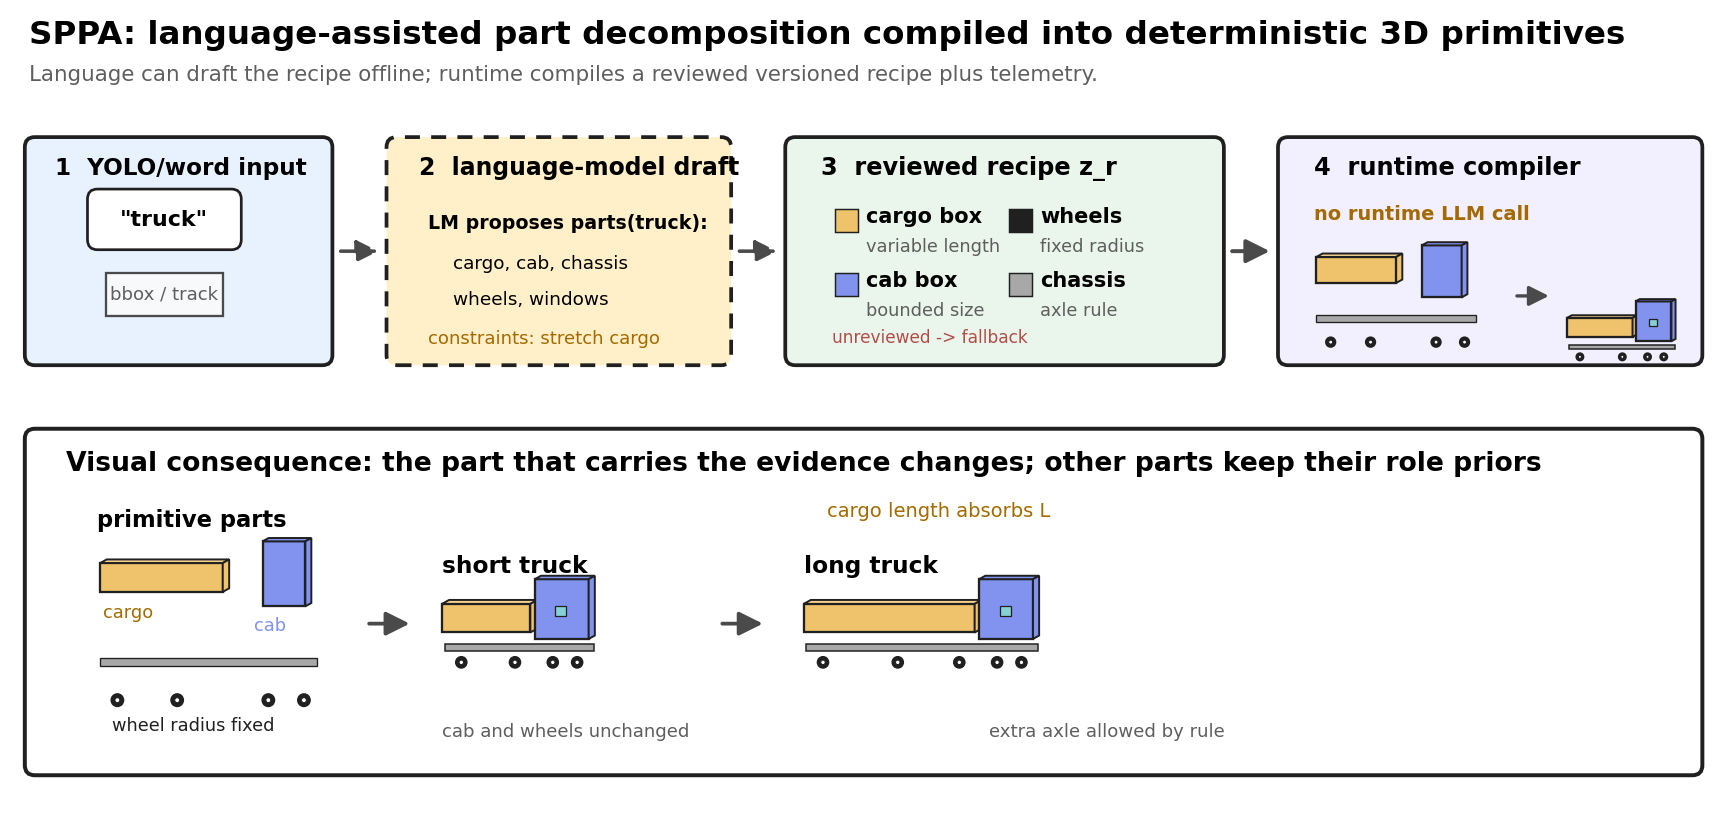
\includegraphics[width=0.9\linewidth]{figures/fig_pipeline_overview.png}
\caption{SPPA semantic-label-to-parts-to-3D mechanism for the truck archetype. A
language model, ontology tool, or human author may draft candidate part roles
offline, but runtime execution uses only a reviewed versioned recipe \(z_r\). An
input label activates an offline draft, the draft is reduced to reviewed part
roles and bounded update rules, and runtime compiles those roles into primitive
geometry. The short and long proxy variants illustrate the implemented
role-specific rule: cargo length changes while cab and wheel priors remain
bounded, so the object is not represented by root-scaling a single box.}
\label{fig:pipeline-overview}
\end{figure}

\section{Related Work}

Text-to-3D and image-to-3D generators target visual asset fidelity from prompts
or images
\cite{poole2022dreamfusion,lin2022magic3d,nichol2022pointe,jun2023shape,tochilkin2024triposr,triposg2025,xu2024instantmesh,stability2024sf3d,sf3d2024,stability2025spar3d,tang2024lgm,wang2024crm,wu2024unique3d,wu2025direct3ds2,lin2025partcrafter,li2026pixal3d,xiang2024trellis,xiang2025trellis2,zhao2025hunyuan3d,hunyuan2025hunyuan3d21,hyper3d2026rodin25}.
SPPA targets a different runtime point: deterministic actor generation from
sparse semantic telemetry, low polygon counts, and cheap per-frame updates.

Monocular and open-vocabulary 3D detection estimate 3D boxes or object state
from images \cite{brazil2022omni3d,yao2024ovmono3d}; YOLOE supplies approximate
open-prompt detection/segmentation evidence rather than universal recognition
\cite{wang2025yoloe}. Animal pose and
reconstruction methods estimate detailed skeletons or category-specific 3D
shape \cite{yu2021ap10k,li20243dfauna,hu2026sam3danimal}. These methods can
provide stronger evidence to SPPA, but SPPA itself is a rendering/backend layer,
not a detector or pose estimator.

Category-conditioned parametric templates are the closest established paradigm.
3D morphable models fit a low-dimensional learned face prior to image
evidence~\cite{blanz1999morphable}, and articulated body and animal models such
as SMPL and SMAL fit a category-conditioned parametric template to scans or
images~\cite{loper2015smpl,zuffi2017smal}. SPPA-MVFit instantiates the same
pattern---a family-conditioned template aligned to observation evidence---with
an eight-part primitive graph and a deliberately shared five-parameter global
alignment. The operating point differs: those models target surface recovery of
a specific category, whereas SPPA targets millisecond, track-updateable display
actors from sparse UAV telemetry, where the contribution is the bounded runtime
contract, the role labels, and the update semantics rather than surface
fidelity.

{\sloppy
Primitive representations have a long history, from volumetric primitives,
recognition-by-components, and superquadrics to learned part decomposition and
neural primitive/CSG parsing
\cite{marr1978representation,biederman1987recognition,solina1990recovery,paschalidou2019superquadrics,tulsiani2017learning,mo2019partnet,fedele2025superdec,ganeshan2026superfrusta,meng2026dualprim,zou20173dprnn,sharma2018csgnet}.
Procedural modeling, shape grammars, and learned shape programs generate or
abstract structured objects from compact programs
\cite{mueller2006procedural,jones2020shapeassembly,jones2023shapecoder,khan2024text2cad,rukhovich2024cadrecode}.
\par}
SPPA uses these ideas operationally, but the claimed novelty is the bounded,
track-updateable semantic telemetry contract inside an Unreal UAV digital twin.

Recent scene-level systems narrow the gap from other directions. SAM 3D
decomposes a single image into composable per-object geometry with layout
\cite{chen2026sam3d}, and PartCrafter generates part-structured meshes from one
image \cite{lin2025partcrafter}; both are heavy offline reconstruction or
generation pipelines, not millisecond telemetry-driven proxies with an update
contract. SuperQuadricOcc reaches real-time semantic occupancy with superquadric
volume rendering in driving scenes \cite{hayes2025superquadricocc}, and
lightweight urban twins render proxy building geometry at interactive rates
\cite{liu2025citygo}; neither constructs role-labeled, metric-scaled object
actors from detector tags and sparse silhouettes. Test-time spatial control
steers generative 3D models with coarse primitives \cite{fedele2025spacecontrol},
which complements rather than replaces a deterministic proxy contract.

Graphics systems already provide level-of-detail, impostors, billboards,
streaming tiles, and virtualized geometry \cite{clark1976hierarchical,decoret2003billboard,epic2026nanite,ogc2023tiles}.
3D and dynamic scene graphs maintain semantic world structure
\cite{armeni2019scenegraph,rosinol2020dynamic,wu2021scenegraphfusion}, and
Hydra-style systems build and optimize hierarchical scene graphs online for
mapping and planning \cite{hughes2022hydra}. SPPA deliberately keeps its own
lightweight contract instead of becoming a node type in such a substrate: a
proxy actor is a display-side object with a bounded descriptor/update payload,
not a mapping layer. Occupancy
grids, OctoMap, ESDF, and TSDF maps support planning and mapping
\cite{hornung2013octomap,oleynikova2017voxblox}. SPPA should be read as a
display actor representation that can consume such upstream evidence, not as a
mapping substrate.

\section{Materials and Methods}

\subsection{The SPPA contract and part graph}

At time \(t\), SPPA consumes an object state
\[
x_t = \{i, \ell, c, b_t, m_t, \xi_t, s_t, \Sigma_t, h_t\},
\]
where \(i\) is a track identifier, \(\ell\) a detector label, \(c\) confidence,
\(b_t\) a bounding region, \(m_t\) an optional mask or footprint, \(\xi_t\) a
world pose estimate, \(s_t\) optional metric dimensions, \(\Sigma_t\)
uncertainty, and \(h_t\) the track history. The resolver maps \(\ell\) to one of
three cases: an \texttt{exact\_class} label with a fixed archetype; a
\texttt{keyword\_archetype} mapping of an out-of-template label to a finite
reviewed archetype, such as vehicle or vertical structure; or a
\texttt{fallback\_unknown\_label} rendered as a generic uncertainty-aware
volume. The versioned recipe manifest covers 23 archetypes and 95 exact or
keyword labels; SPPA can accept an open detector tag at runtime, but the tag is
normalized into a reviewed family or a conservative unknown fallback before
geometry is emitted.

Each archetype \(a\) defines a part graph
\[
G_a = (V_a,E_a), \quad v_k = (p_k,r_k,\tau_k,\rho_k),
\]
where \(p_k\) is a primitive type, \(r_k\) is its role, \(\tau_k\) its transform
relative to the actor root, and \(\rho_k\) role-specific parameters such as
dimension priors, color/material role, and confidence tags. The current
implementation uses boxes, cylinders, ellipsoids, cones, and tori
(Figure~\ref{fig:family-graphs}).

\begin{figure}[H]
\centering
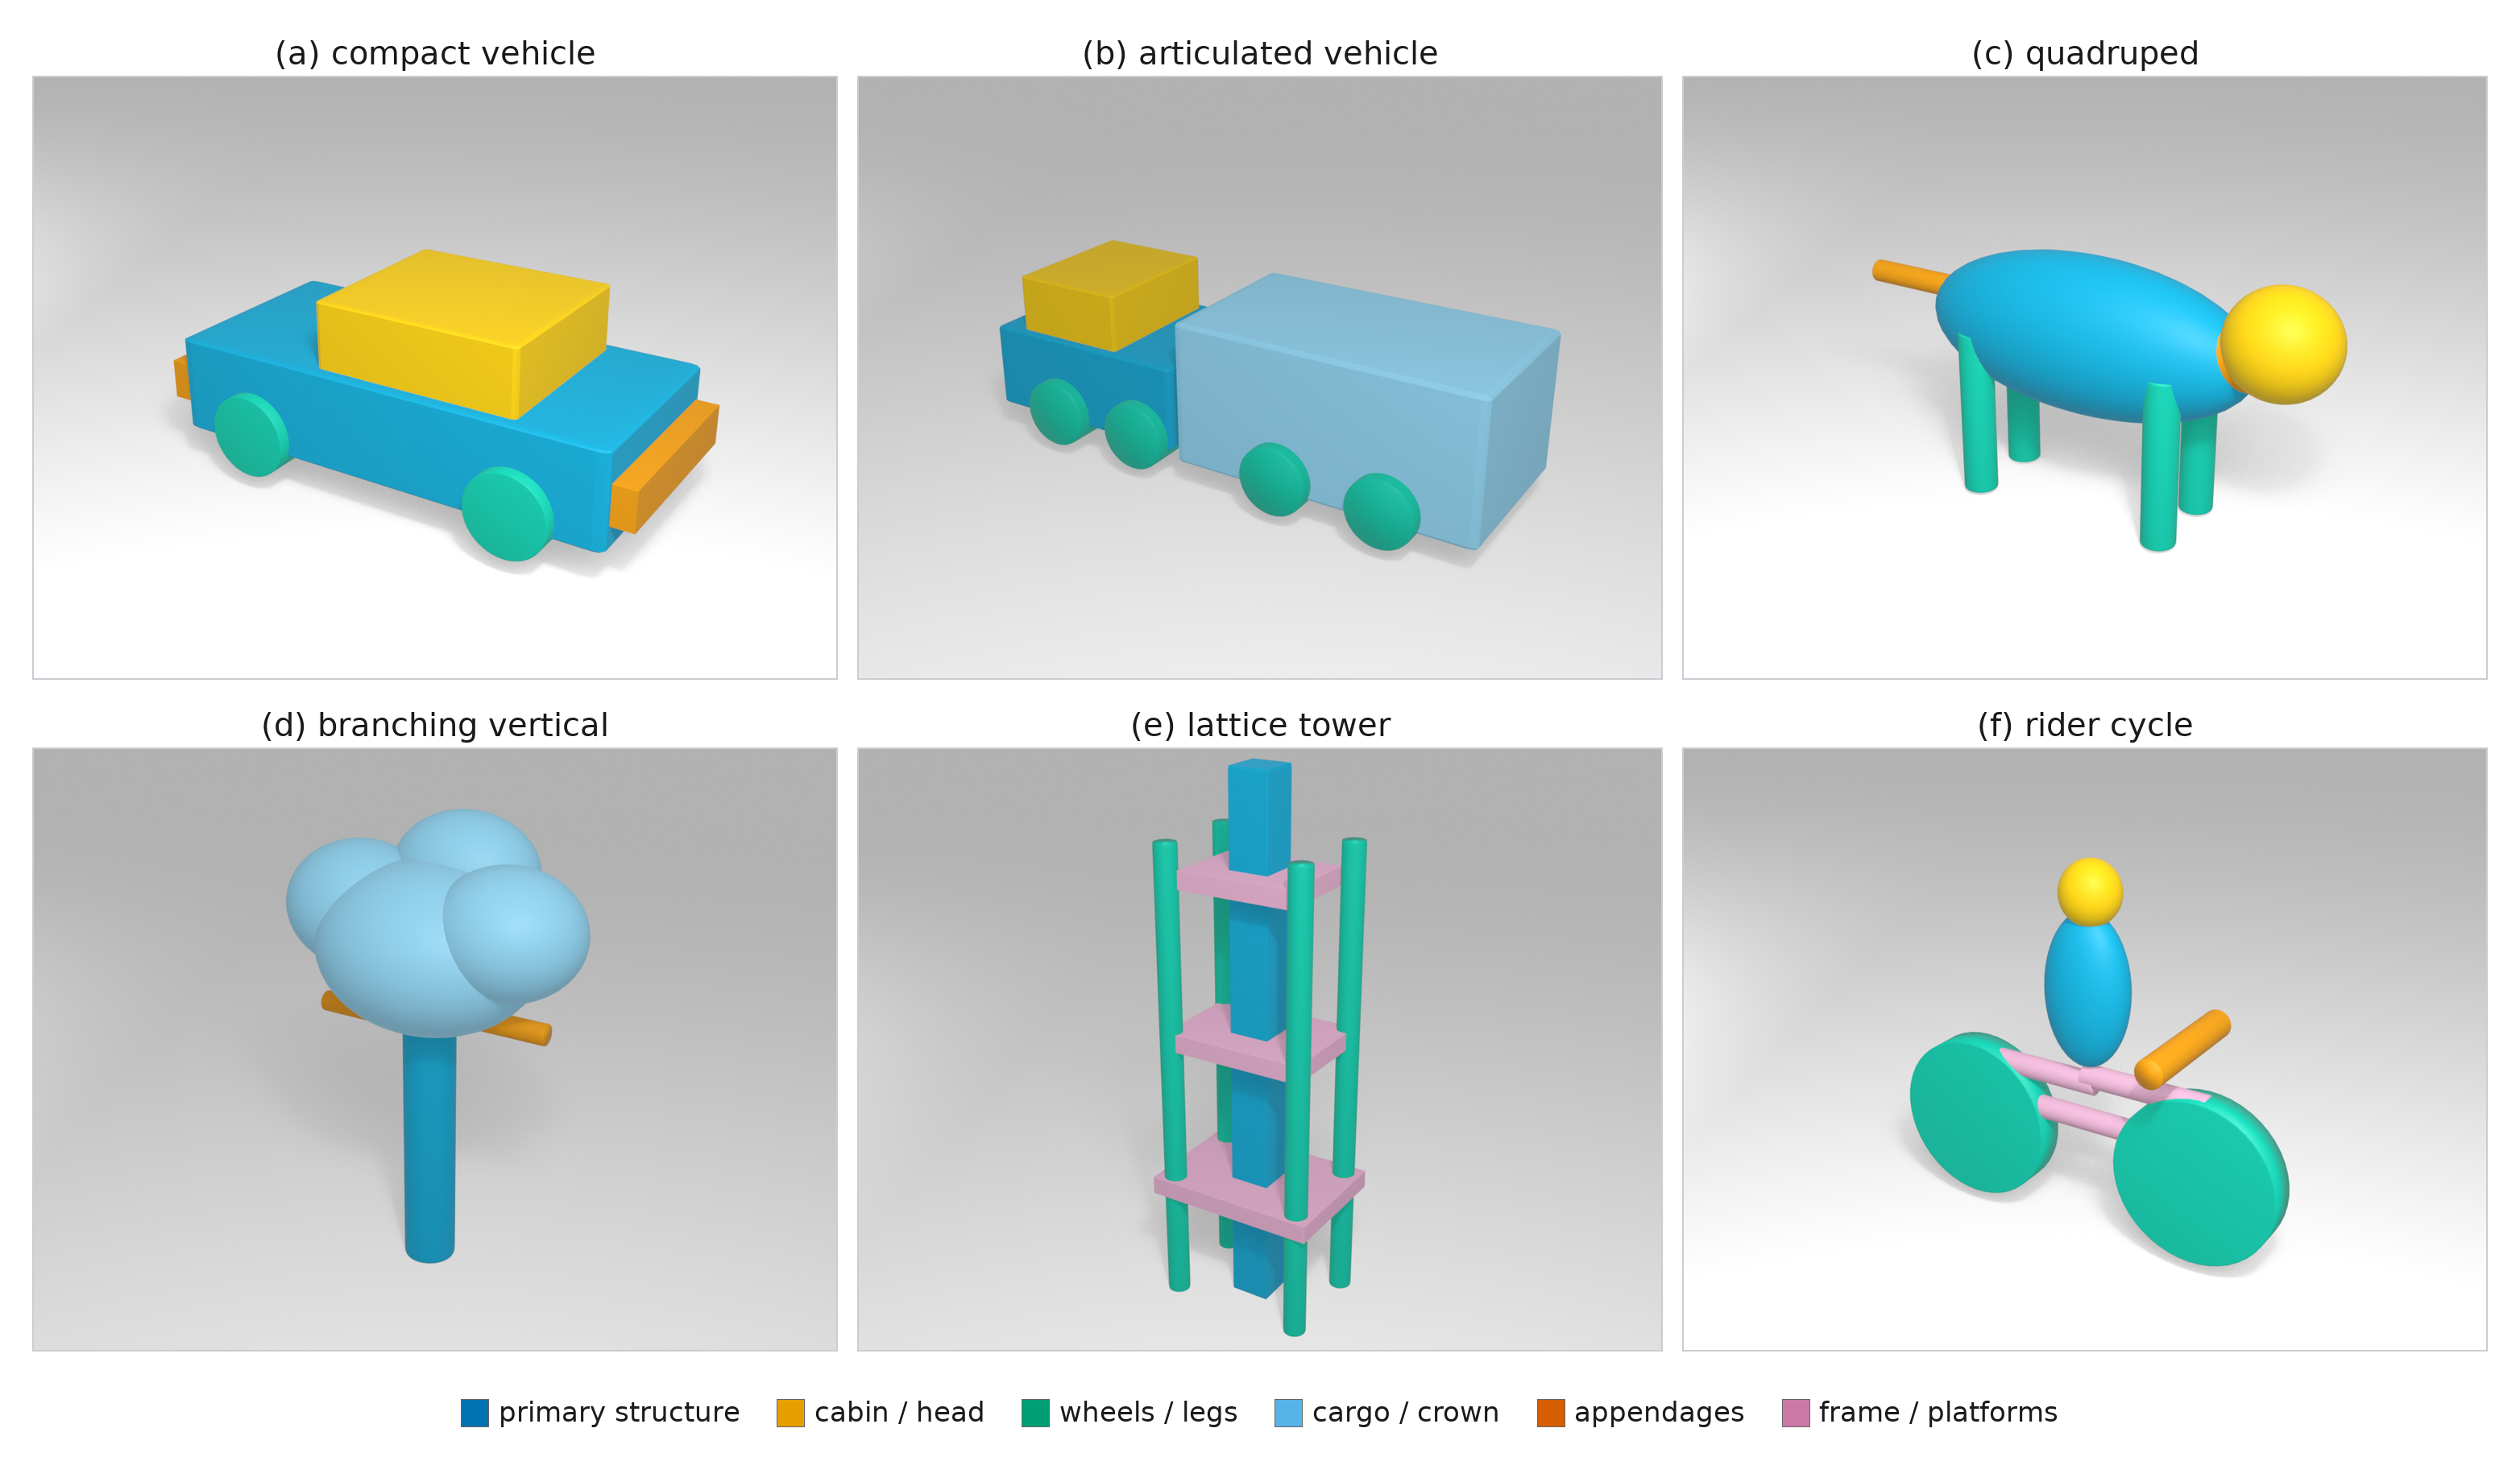
\includegraphics[width=0.8\linewidth]{figures/fig_family_graphs_blender.png}
\caption{The six benchmark family part graphs used by SPPA-MVFit
(\texttt{compact\_vehicle}, \texttt{articulated\_vehicle}, \texttt{quadruped},
\texttt{branching\_vertical}, \texttt{lattice\_tower}, \texttt{rider\_cycle}):
eight primitive slots per family with role-conditioned priors; colors denote
semantic roles.}
\label{fig:family-graphs}
\end{figure}

Vehicle adaptation is the clearest implemented case. A long truck and a short
truck should not be produced by globally scaling the same box. In the current
vehicle grammar, cab and wheel dimensions remain bounded by role priors, while
the cargo/body span and axle placement absorb length changes. In the synthetic
truck check, two descriptors with equal width/height and different length keep
cab scale fixed at \([1.656,2.070,1.952]\) m and wheel scale fixed at
\([0.392,0.094]\) m, while cargo/body length changes from \(2.263\) m to
\(5.188\) m.

\paragraph{Language model use (offline only).}
A language model, ontology tool, or human author may propose candidate part
decompositions offline; those candidates must be reviewed, versioned, and
regression tested before admission. No language model is called at runtime.

\paragraph{Pose, yaw, and updates.}
The descriptor separates actor pose \(\xi_t\) from part parameters \(q_t\). Pose
changes are per-frame updates; topology regeneration is avoided unless the
class/archetype changes or new evidence crosses a configured threshold. Yaw
ambiguity is handled explicitly: a top-down footprint or PCA orientation gives
an axial orientation modulo \(\pi\), and signed yaw requires velocity,
asymmetry, multi-frame evidence, or an external heading source; otherwise the
descriptor sets \texttt{yaw\_ambiguous=true}.

\subsection{End-to-end pipeline: two input paths, one builder}
\label{sec:pipeline}

Both input contracts terminate in the same deterministic builder; they differ
only in how much evidence reaches the recipe. The tag/text path compiles a
reviewed recipe at its prior dimensions: normalize the label through the
reviewed ontology, select the frozen part graph \(G_a\) and its prior role
parameters, emit role-labeled primitives with connector cylinders for
semantically attached parts, and emit the versioned descriptor consumed once
per track by the renderer. The detector/image path inserts four evidence
stages before the same builder: (1)~\textbf{Observe}---detector label,
confidence, bbox, and native mask polygon are stored in a
\texttt{SPPA-OBS-0.1} record with declared camera/flight geometry and a
covariance-style uncertainty envelope; (2)~\textbf{Project}---the mask polygon
is projected through the declared camera model into an oriented ground
footprint, keeping the axis-aligned mask box and a PCA axial orientation as
audit evidence; (3)~\textbf{Scale}---with declared metric calibration the
footprint becomes a metric length/width/height proposal; without calibration
the mask remains image-space evidence and cannot change metric geometry;
(4)~\textbf{Gate}---a class-aware constraint-fusion step accepts plausible
scale, clamps implausible length/width ratios through the family aspect prior,
withholds unsafe image-derived pose/yaw from the runtime descriptor, and
records every decision with its reason. Because both paths share the builder
and the descriptor contract, their outputs are directly comparable
(Figure~\ref{fig:role-colored}).

\begin{figure}[H]
\centering
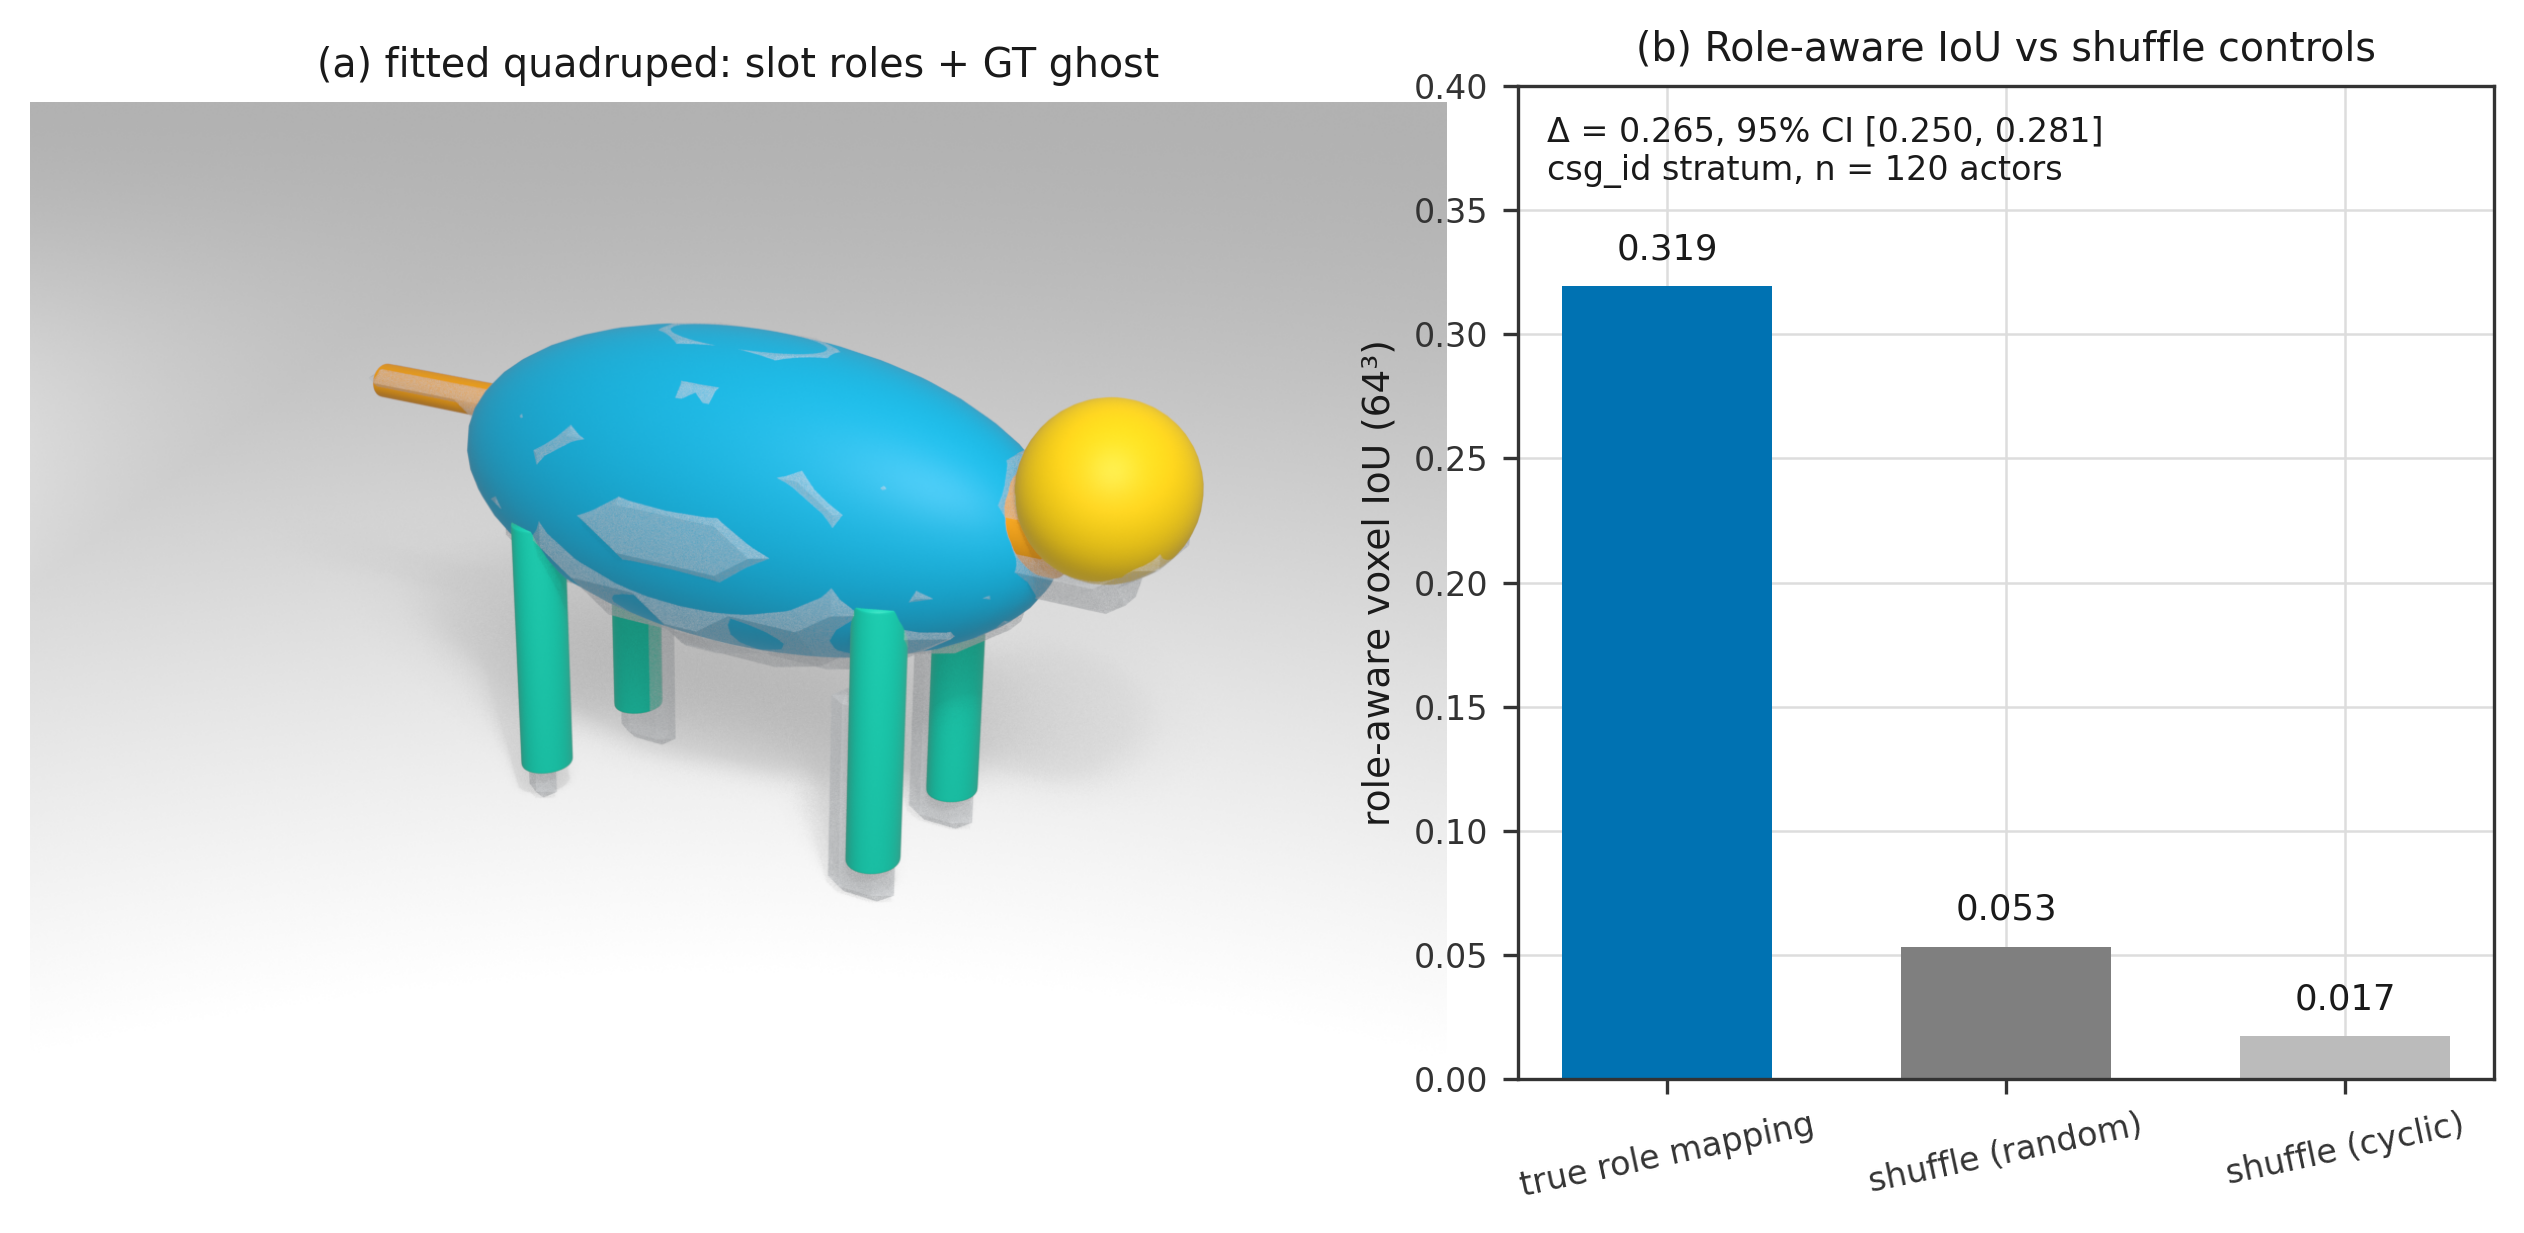
\includegraphics[width=0.5\linewidth]{figures/fig_role_colored_blender.png}
\caption{(a) A built SPPA proxy with primitives colored by semantic role. Role
labels are part of the emitted actor contract: they drive bounded per-role
update rules, material/uncertainty tags, and the connector primitives between
semantically attached parts. (b) Role-aware IoU of the fitted proxies against
random-shuffle and cyclic-shuffle controls (\(0.319\) versus \(0.053\) and
\(0.017\); Section~4.5).}
\label{fig:role-colored}
\end{figure}

\paragraph{Worked example (tractor-trailer probe).}
The real crop yields YOLOE evidence \texttt{vehicle} at confidence 0.47 with a
54-point native mask. Projection proposes a raw footprint of
\(16.85\times6.21\times3.40\) m; the gate applies soft low-confidence fusion,
clamps the footprint through the vehicle aspect prior to
\(12.11\times3.76\times3.40\) m, withholds image-derived pose, and refines the
weak label only to the conservative \texttt{articulated\_vehicle} family. The
shared builder then emits a 1{,}904-triangle proxy (Supplementary
Section~S.4).

\subsection{Descriptor and runtime backend}
\label{sec:implementation}

A \texttt{SPPA-DESC-0.2} record stores resolver source, match type, fallback
reason, scale source, mask footprint evidence, yaw ambiguity, shape confidence,
material source, part list, primitive counts, and scheduler metadata; a
\texttt{SPPA-UPD-0.2} record separates create/regenerate payloads from
pose/no-op/shape updates, and \texttt{descriptor\_id} acts as a topology-cache
identity so that a pose update never looks like a new mesh descriptor. The
design goal is to generate once per track/archetype, update
pose/material/uncertainty every frame, and apply shape-parameter changes in
place when the part topology is unchanged. An optional Unreal Engine 5.7
backend ingests the same descriptors alongside curated assets, which remain
the default; the SPPA backend constructs primitive components from the
\texttt{parts} array, applies update packets, and rejects invalid JSON or
mismatched descriptor identifiers without changing the current actor.

\subsection{Confirmatory protocol}
\label{sec:mvfit}

Every compared method receives the same case identifier, morphology-family
token, metric world box, and two \(96\times 96\) orthographic binary
silhouettes (top and side). No method receives RGB pixels, detector scores,
source parameters, ground-truth occupancy, evaluation projections, or real or
replay telemetry. An actor is an ordered list of eight primitive slots (boxes,
cylinders, ellipsoids). Family graphs and a single \texttt{generic} graph are
stored as static JSON. The only builder used by text-only SPPA, Generic-MVFit,
and SPPA-MVFit is
\begin{equation}
A = \mathrm{Build}(g,\theta),\qquad
\theta=(\log s_x,\log s_y,\log s_z,s_{\mathrm{sec}},o_{\mathrm{sec}}),
\end{equation}
with identical bounds for every graph \(g\). Text-only SPPA uses the family
graph at the default \(\theta_0\). Generic-MVFit and SPPA-MVFit optimize the
same five parameters with the same silhouette disagreement objective---the
mean top/side disagreement
\(0.5(1-\mathrm{IoU}_{\mathrm{top}})+0.5(1-\mathrm{IoU}_{\mathrm{side}})\) plus
a small centering regularizer---using a coordinate descent over three
shrinking step fractions that evaluates exactly 31 objective values; only the
graph identity differs (\texttt{generic} vs family). Baselines include
axis-aligned box, ellipsoid, capsule, billboard, and nonsemantic visual hull
from the same masks. The fitter is deliberately a five-parameter global
alignment shared by all slots; the contribution is the family-conditioned
representation and the runtime contract, not the optimizer
(Figure~\ref{fig:fitting-sequence}).

\begin{figure}[H]
\centering
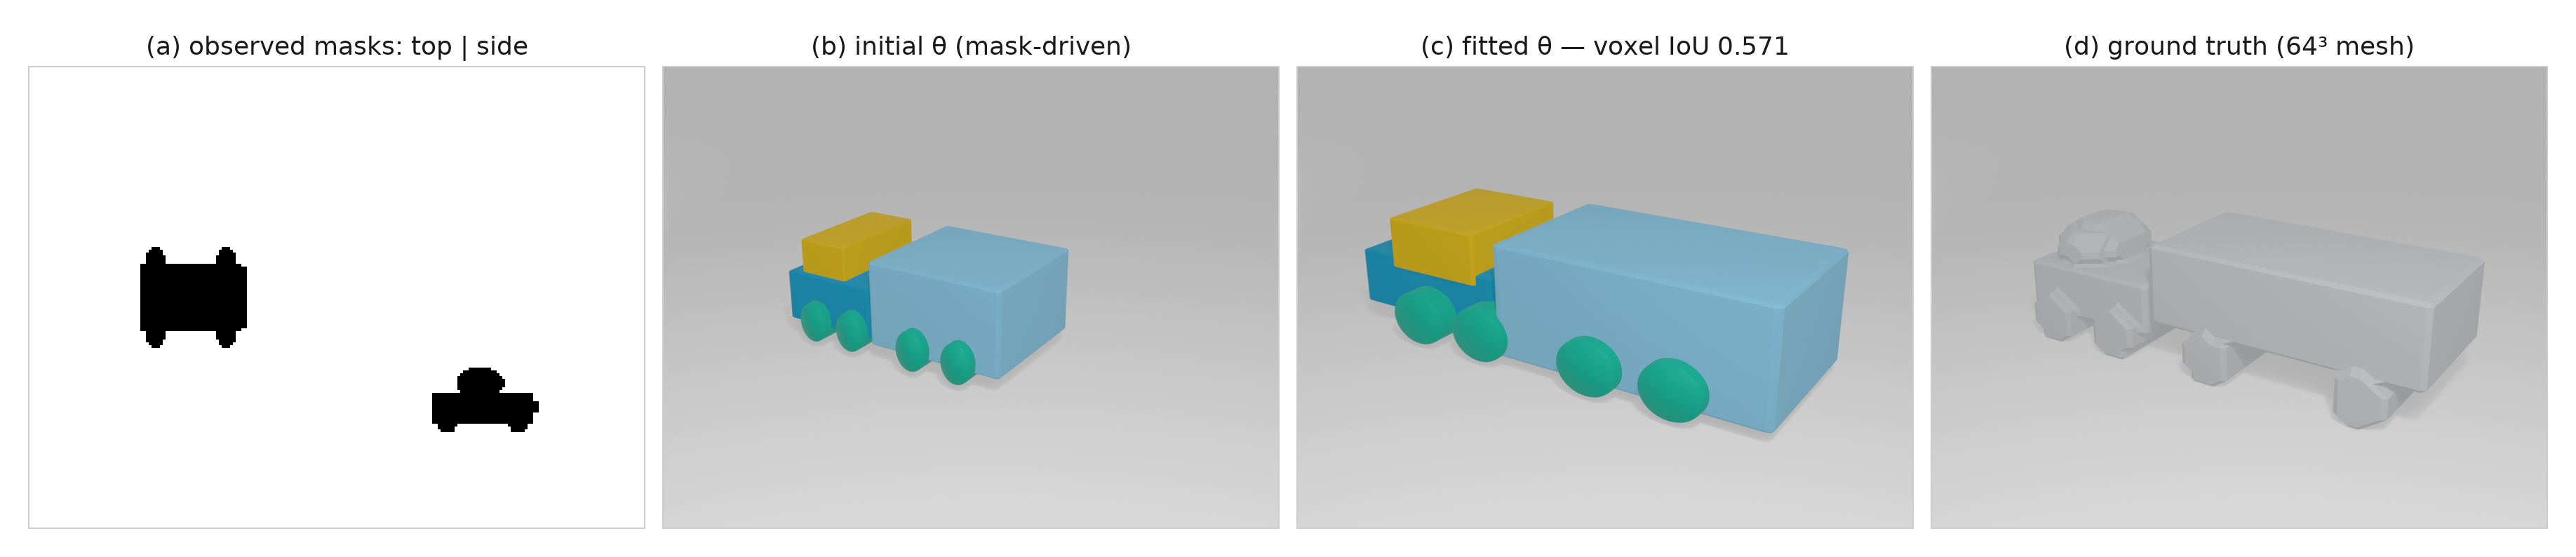
\includegraphics[width=0.8\linewidth]{figures/fig_fitting_sequence_blender.png}
\caption{Fitting of SPPA-MVFit on a held-out actor: (a)~the observed
silhouette pair, (b)~initialization from the observed mask extents,
(c)~the converged eight-part proxy, and (d)~the ground-truth voxel mesh.}
\label{fig:fitting-sequence}
\end{figure}

The \texttt{generic} graph was designed by the authors as a plausible
family-agnostic prior: eight symmetric ellipsoid slots with no
family-specific topology, proportions, or role labels, frozen before the
benchmark was run. It is hand-crafted, not learned, not random, and not the
mean of the six family graphs. Because the same team authored the family
graphs and this generic competitor, three alternative generic graphs were
registered in writing before any measurement and are evaluated in
Section~\ref{sec:generic-sensitivity}; the shared-authorship threat is
discussed in Section~\ref{sec:threats}.

The primary hypothesis compares clean-mask 64-cubed voxel IoU of SPPA-MVFit
against Generic-MVFit. Analysis units are 240 source actors (20 per family in
each of two strata). The confirmatory estimand is the equal-stratum mean paired
difference. H1 passes only if the lower endpoint of a two-sided 95\% stratified
actor-bootstrap percentile interval (10{,}000 resamples, seed 77157) exceeds
\(+0.030\). The margin and the power analysis behind the sample size were fixed
before evaluation: with paired-difference SD \(0.12\), \(n{=}240\) actors give
approximately 90\% normal-approximation power to distinguish a true mean of
\(+0.055\) from the \(+0.030\) margin. The full protocol was preregistered
and sealed before evaluation; the seed provenance, amendment log, and freeze
records are given in the supplement. Development results
were used only to implement the frozen package and are not confirmatory.

Source actors come from two strata: CSG-ID unions of solids with family
topology, and implicit-OOD occupancy from superelliptic extrusions,
taper/twist, toroidal sections, and spline-distance tubes. Source and method
modules do not import each other. The held-out set is developer-held-out
synthetic geometry, not an externally blinded public UAV benchmark.

All confirmatory and post-hoc fits ran on one benchmark workstation (AMD
Zen~5, 32 logical CPUs, Windows~11, CPython 3.12.6); the external
neural-generator runs of Section~\ref{sec:neural-external-wave} used an
RTX~5090 32~GB GPU on the same machine.

\subsection{Evaluation data}
\label{sec:evaluation-data}

The synthetic benchmark covers six families selected before freezing for
morphological coverage of the ground-object envelope a UAV twin must display:
compact rigid bodies (\texttt{compact\_vehicle}), elongated articulated bodies
(\texttt{articulated\_vehicle}), legged organic forms (\texttt{quadruped}),
branching vertical growth (\texttt{branching\_vertical}), thin lattice
structures (\texttt{lattice\_tower}), and rider-plus-cycle combinations
(\texttt{rider\_cycle}), with 20 actors per family in each of the two strata
(\(n{=}240\)). A post-hoc exploratory drop-one-family re-analysis
(Section~\ref{sec:results-decomposition}) confirms the headline difference is
not carried by any single family: excluding any one family leaves the paired
difference between \(0.152\) and \(0.214\), always above the \(+0.030\)
margin. As an external case study outside the design distribution, the same
methods were run on \(n{=}52\) real third-party meshes (Objaverse LVIS subset
and ModelNet40) under a class-to-family mapping frozen in writing before any
evaluation (Section~\ref{sec:external-sanity}). Four real-image probes (a road
cyclist, a mountain electrical tower, a mountain tractor, and a tractor with
trailer) exercise the dual-input contract of Section~\ref{sec:pipeline} with a
YOLOE-26s open-vocabulary detector (checkpoint \texttt{yoloe-26s-seg.pt}) as
approximate semantic evidence (Section~\ref{sec:deployment-summary}).

\section{Results}
\label{sec:primary-results}

\subsection{Primary confirmatory result}

Table~\ref{tab:mvfit-h1} reports the confirmatory decision: H1 passes, with
mean \(\Delta\mathrm{IoU}=0.190\) and 95\% CI \([0.181,0.199]\). The CSG-ID
stratum mean difference is \(0.209\) and the implicit-OOD stratum mean
difference is \(0.172\); neither is non-positive, so a cross-stratum
generalization warning is not triggered by the protocol rule.
Figure~\ref{fig:h1-by-family} shows the paired difference in every
family-by-stratum cell (per-cell values in Supplementary Section~S.9); all
twelve cells are positive, and the smallest gain is the compact-vehicle
implicit-OOD cell.

\begin{table}[H]
\centering
\footnotesize
\caption{Preregistered primary endpoint on the held-out synthetic test
(\(n{=}240\) actors). Provenance: \texttt{synthetic\_geometry}. H1 passes only
if the stratified bootstrap 95\% lower bound exceeds \(+0.030\).}
\label{tab:mvfit-h1}
\input{benchmarks/results/sppa_mvfit_h1_summary.tex}
\end{table}

\begin{figure}[H]
\centering
\begin{minipage}{0.48\linewidth}
\centering
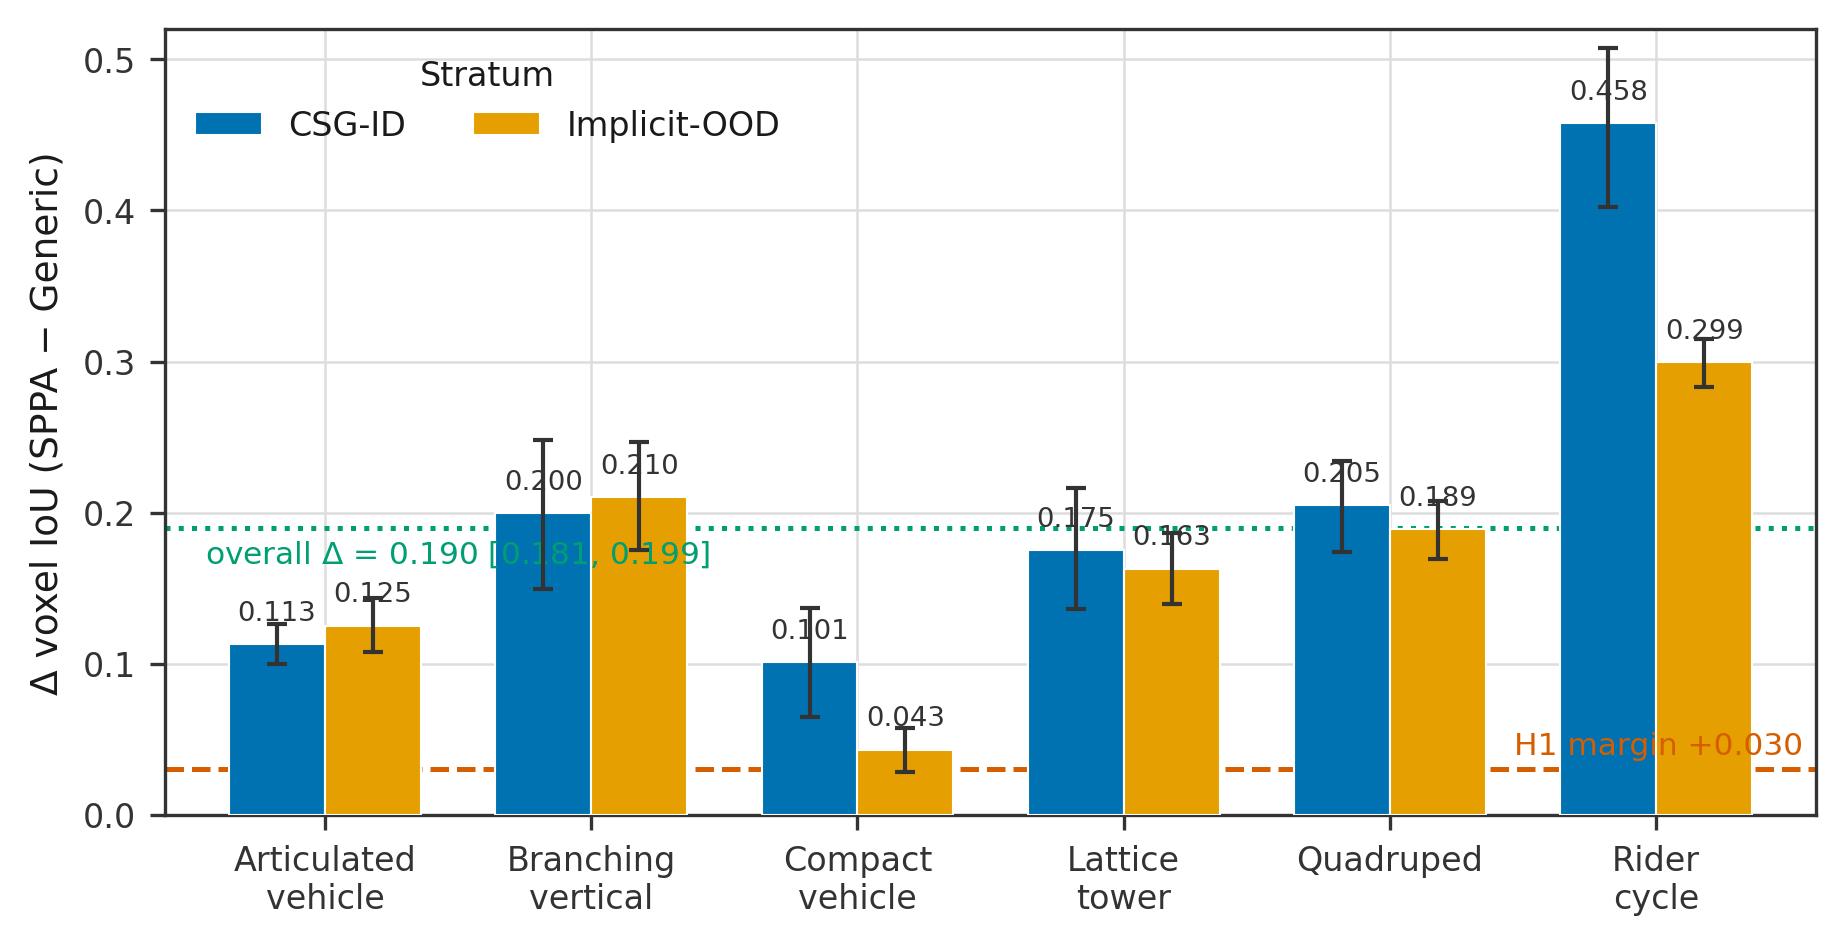
\includegraphics[width=\linewidth]{figures/fig_h1_by_family.png}
\caption{Paired clean-mask mean IoU difference of SPPA-MVFit minus
Generic-MVFit by morphology family and source stratum (\(n{=}240\)). All
twelve cells are positive; the equal-stratum aggregate is the primary
estimate of Table~\ref{tab:mvfit-h1}.}
\label{fig:h1-by-family}
\end{minipage}\hfill
\begin{minipage}{0.48\linewidth}
\centering
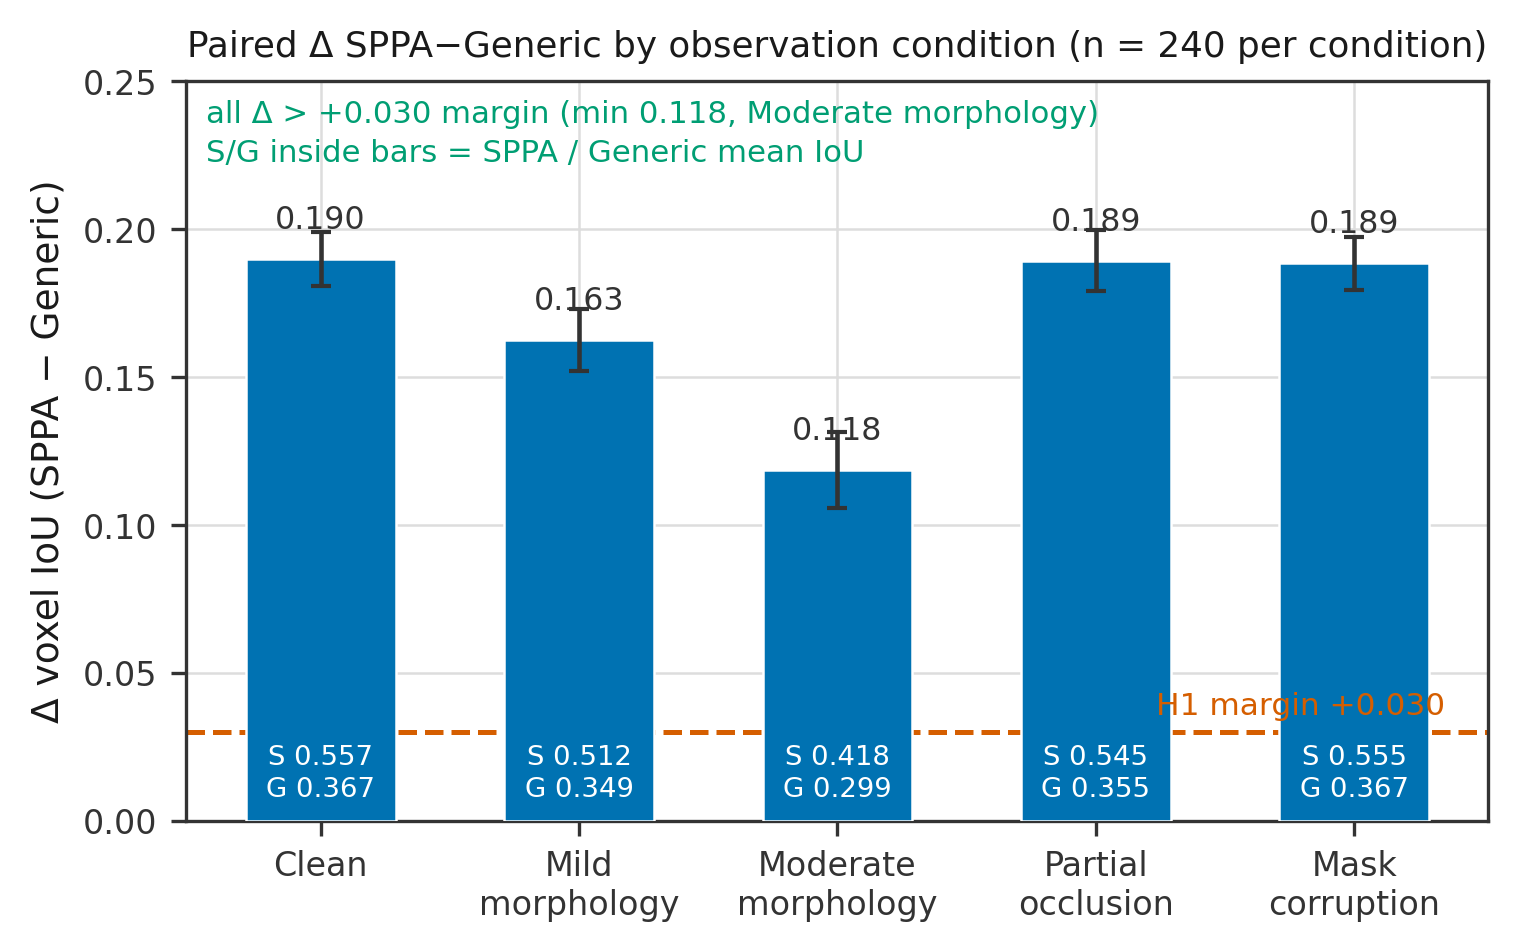
\includegraphics[width=\linewidth]{figures/fig_robustness_conditions.png}
\caption{Paired SPPA-MVFit minus Generic-MVFit mean IoU difference with 95\%
bootstrap intervals under the five prespecified observation conditions
(\(n{=}240\) per condition). The dashed line marks the prespecified
\(+0.030\) margin; it is exceeded under every condition.}
\label{fig:robustness-conditions}
\end{minipage}
\end{figure}

Table~\ref{tab:mvfit-means} reports clean-condition method means and
wall-clock costs, and Table~\ref{tab:mvfit-secondary} the paired differences
of SPPA-MVFit against the remaining baselines under the same stratified
bootstrap construction. SPPA-MVFit exceeds SPPA text-only (mean
\(\Delta=0.130\), CI \([0.116,0.144]\)) and all lightweight geometric
baselines. Mean IoU of SPPA-MVFit (\(0.557\)) is slightly above nonsemantic
visual hull~\cite{laurentini1994visual} (\(0.522\)), but visual hull is denser
occupancy geometry without a role-labeled lightweight actor contract, so it is
not presented as a defeated runtime competitor. Median single-call descriptive
SPPA-MVFit time is \(9.4\)~ms (p95 \(10.6\)~ms), below the secondary
local-cost gates of 100~ms median / 250~ms p95. A resolution-sensitivity check
at grids 48/64/80 on the prespecified actor subset reports paired differences
of \(0.198\), \(0.197\), and \(0.188\), with maximum deviation
\(|\Delta|\le 0.0094\), below the \(0.015\) protocol threshold. The secondary
intervals in Table~\ref{tab:mvfit-secondary} are per-comparison intervals and
are not adjusted for multiplicity; confirmatory inference in this paper is H1
only.

\begin{table}[H]
\centering
\footnotesize
\caption{Clean-mask method summary on the held-out test (\(n{=}240\)). Mean/median
are 64-cubed voxel IoU. Timings are single-call wall-clock milliseconds on the
benchmark machine and are not Unreal frame times.}
\label{tab:mvfit-means}
\begin{tabular}{@{}lrrrr@{}}
\toprule
Method & Mean IoU & Median IoU & Median ms & p95 ms \\
\midrule
SPPA-MVFit & 0.557 & 0.563 & 9.43 & 10.60 \\
Generic-MVFit & 0.367 & 0.390 & 11.34 & 11.81 \\
SPPA text-only & 0.427 & 0.441 & 0.77 & 1.81 \\
Visual hull & 0.522 & 0.567 & 0.22 & 0.24 \\
Ellipsoid & 0.342 & 0.292 & 0.50 & 0.55 \\
Capsule & 0.325 & 0.260 & 0.95 & 1.07 \\
Axis-aligned box & 0.248 & 0.190 & 0.23 & 0.27 \\
Billboard & 0.173 & 0.148 & 0.23 & 0.26 \\
\bottomrule
\end{tabular}

\end{table}

\begin{table}[H]
\centering
\footnotesize
\caption{Paired clean-mask mean IoU differences of SPPA-MVFit minus each
comparator (stratified actor bootstrap 95\% intervals, per-comparison and
unadjusted across secondary endpoints). Visual hull is a
high-complexity geometry reference, not a lightweight runtime actor.}
\label{tab:mvfit-secondary}
\begin{tabular}{@{}lrrr@{}}
\toprule
Comparator & Mean $\Delta$ IoU & 95\% CI low & 95\% CI high \\
\midrule
Generic-MVFit (H1) & 0.190 & 0.181 & 0.199 \\
SPPA text-only & 0.130 & 0.116 & 0.144 \\
Visual hull & 0.036 & 0.027 & 0.044 \\
Ellipsoid & 0.216 & 0.207 & 0.224 \\
Capsule & 0.233 & 0.224 & 0.241 \\
Axis-aligned box & 0.310 & 0.301 & 0.318 \\
Billboard & 0.384 & 0.375 & 0.393 \\
\bottomrule
\end{tabular}

\end{table}

\subsection{Robustness under corrupted observations and failure analysis}
\label{sec:robustness}

The prespecified observation conditions---mild and moderate mask noise,
partial occlusion, and moderate morphology corruption---were fixed in the
protocol and evaluated with the confirmatory run
(Figure~\ref{fig:robustness-conditions}; per-condition table in Supplementary
Section~S.9). The margin is exceeded under all five conditions, including
moderate morphology corruption (\(\Delta=0.118\), CI \([0.106,0.131]\)).
Moderate morphological corruption degrades the margin far more than mask
corruption or partial occlusion (\(\Delta=0.189\) each): evidence that
contradicts the graph prior hurts the fit more than missing or noisy evidence.


Exactly \(5\) of \(240\) clean cases fall below the prespecified failure
threshold (voxel IoU \(<0.25\)); all five are \texttt{lattice\_tower} CSG-ID
cases (worst \(0.147\) and \(0.148\)). Inspection attributes the failures to
sub-voxel geometry: the failing towers have leg and plate thicknesses of
\(0.09\)--\(0.37\) world units against a \(0.15\times0.10\times0.10\) voxel
cell, and the seven actor methods score at most \(0.24\) on these actors
(visual hull at most \(0.43\))---a resolution effect shared by every method,
not a family-prior failure. Convergence telemetry supports the same reading:
\(88.7\%\) of SPPA-MVFit cases still improve in the final sweep and its
\(\theta\) never sits at the frozen bounds, whereas Generic-MVFit pins
\(\theta\) at a bound in \(57.9\%\) of cases---evidence of a mismatched prior
demanding out-of-range excursions, not of SPPA overfitting. Surface metrics
agree with the volume ranking: Chamfer
distance \(0.008\) for SPPA-MVFit versus \(0.009\) for visual hull and
\(0.016\) for Generic-MVFit (Supplementary Section~S.9), and F-score at
1.5 voxels of \(0.831\) versus
\(0.799\) and \(0.560\) respectively
(Table~\ref{tab:surface-metrics}).

\begin{table}[H]
\centering
\footnotesize
\caption{Surface metrics on the clean condition
(\(n{=}240\)). F-score at a 1.5-voxel threshold against ground-truth
surfaces; paired differences versus SPPA-MVFit with stratified bootstrap
95\% intervals.}
\label{tab:surface-metrics}
\begin{tabular}{@{}lrrrr@{}}
\toprule
Method & F-score$@1.5$ vox & $\Delta$ vs SPPA & 95\% CI \\
\midrule
SPPA-MVFit & 0.831 & --- & --- \\
Generic-MVFit & 0.560 & $-$0.271 & [$-$0.280, $-$0.262] \\
Visual hull & 0.799 & $-$0.032 & [$-$0.040, $-$0.023] \\
SPPA text-only & 0.706 & $-$0.125 & [$-$0.140, $-$0.110] \\
\bottomrule
\end{tabular}

\end{table}

\subsection{Representation versus fitting: the graph-by-fitting decomposition}
\label{sec:results-decomposition}

A post-hoc exploratory analysis completes the graph-by-fitting factorial
(Figure~\ref{fig:2x2-decomposition}): the previously missing cell, the generic
graph at the default \(\theta_0\), scores \(0.180\). The family graph with no
fitting at all (\(0.427\)) already exceeds the fully fitted generic
competitor (\(0.367\)). Fitting adds \(+0.187\) on the generic graph and
\(+0.130\) (CI \([0.117,0.143]\)) on the family graph, with a negative
interaction (\(-0.058\)). The H1 headline therefore decomposes into a larger
representation effect---graph effect at no fit \(+0.248\), CI
\([0.234,0.261]\)---plus a smaller fitting contribution on top of it, and the
claim of this paper is accordingly about the family-conditioned
representation, not about fitter sophistication. The drop-one-family
re-analysis of Section~\ref{sec:evaluation-data} and the per-stratum effect
estimates are tabulated in Supplementary Section~S.9.

\begin{figure}[H]
\centering
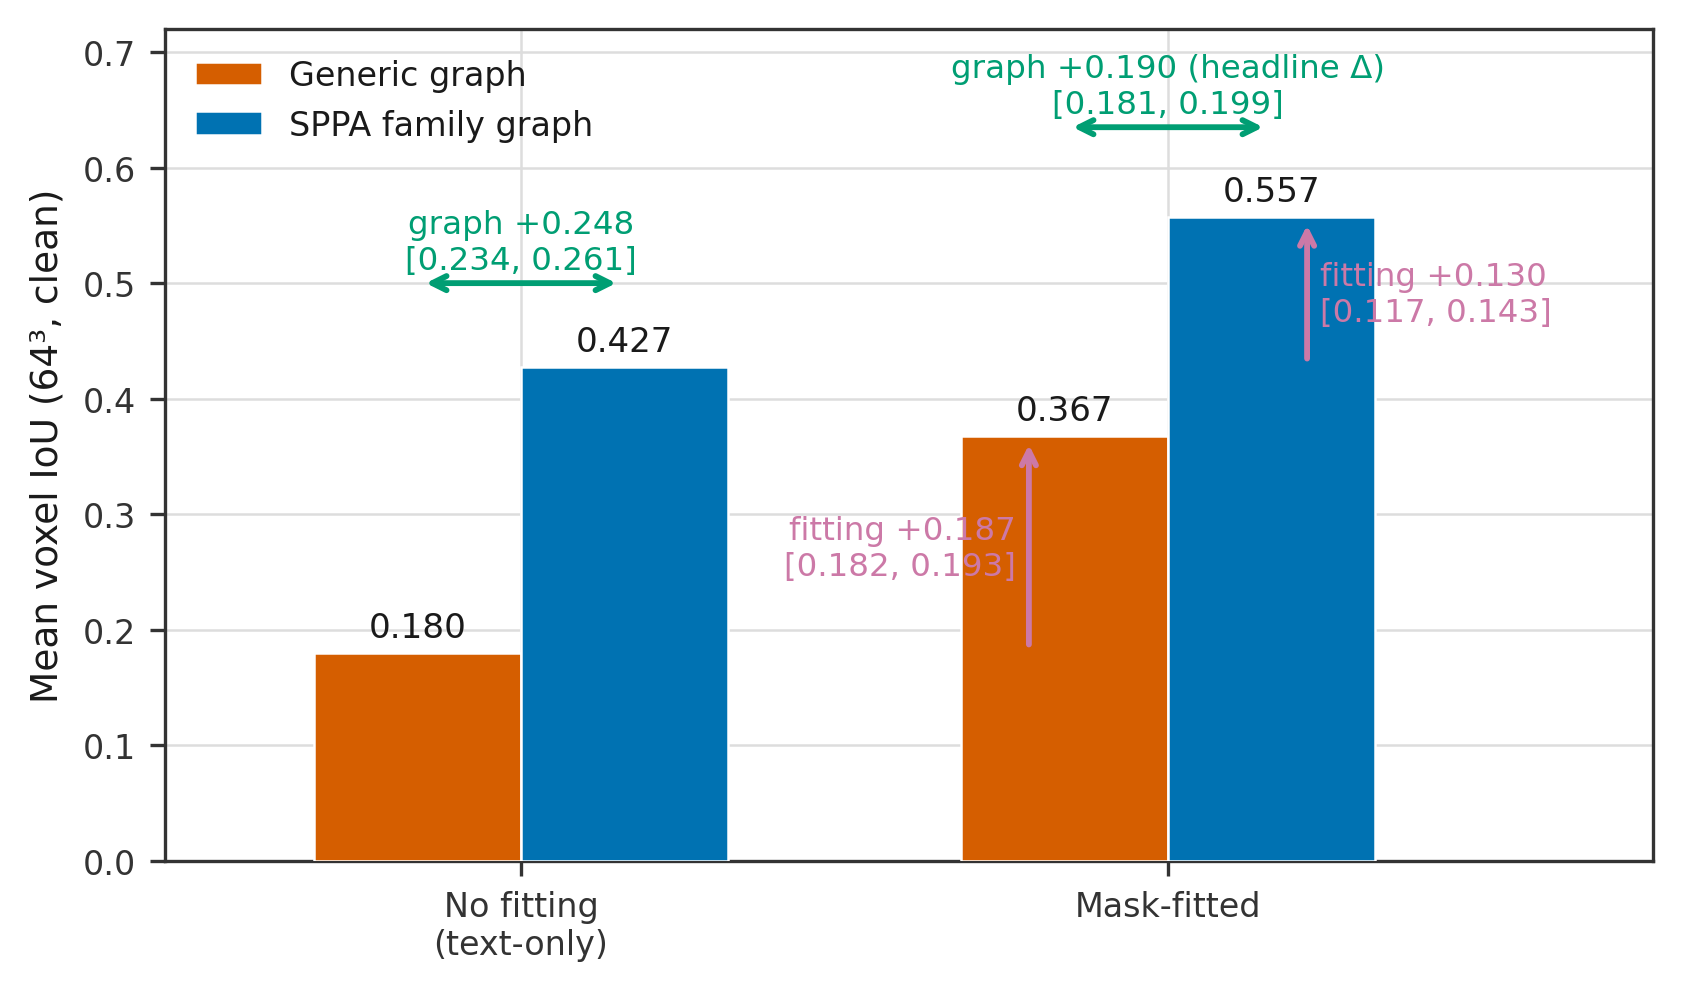
\includegraphics[width=0.5\linewidth]{figures/fig_2x2_decomposition.png}
\caption{Graph-by-fitting \(2\times2\) decomposition (clean condition,
\(n{=}240\), mean voxel IoU). Rows: graph (\texttt{generic} vs family);
columns: no fitting (\(\theta_0\)) vs 31-candidate silhouette fitting. The
family graph without fitting already exceeds the fitted generic graph.}
\label{fig:2x2-decomposition}
\end{figure}

\subsection{Wrong-family tokens}
\label{sec:wrong-family}

The confirmatory benchmark supplies the correct family token, so it does not
measure the principal failure mode of a family-conditioned method. Each
held-out actor was therefore also fitted under each of the five incorrect
family tokens (1{,}200 additional deterministic fits through the same fitting
path; Figure~\ref{fig:wrong-family-matrix}). A wrong token is far worse than
no family prior at all: the wrong-token mean is \(0.205\) against
Generic-MVFit \(0.367\), a paired difference of \(-0.162\) (CI
\([-0.167,-0.158]\)), with \(98.3\%\) of actors scoring below their own
generic fit, and even the per-actor \emph{best} wrong token (\(0.361\)) does
not beat the generic mean. The deployed contract already routes unsupported
labels to a generic fallback volume and refines low-confidence detector labels
only to conservative families; this result makes the symmetric design
implication explicit---a family token should be accepted only with adequate
detector confidence or agreement, and otherwise the fit should degrade to the
generic graph rather than commit to a mismatched family.

\begin{figure}[H]
\centering
\begin{minipage}{0.52\linewidth}
\centering
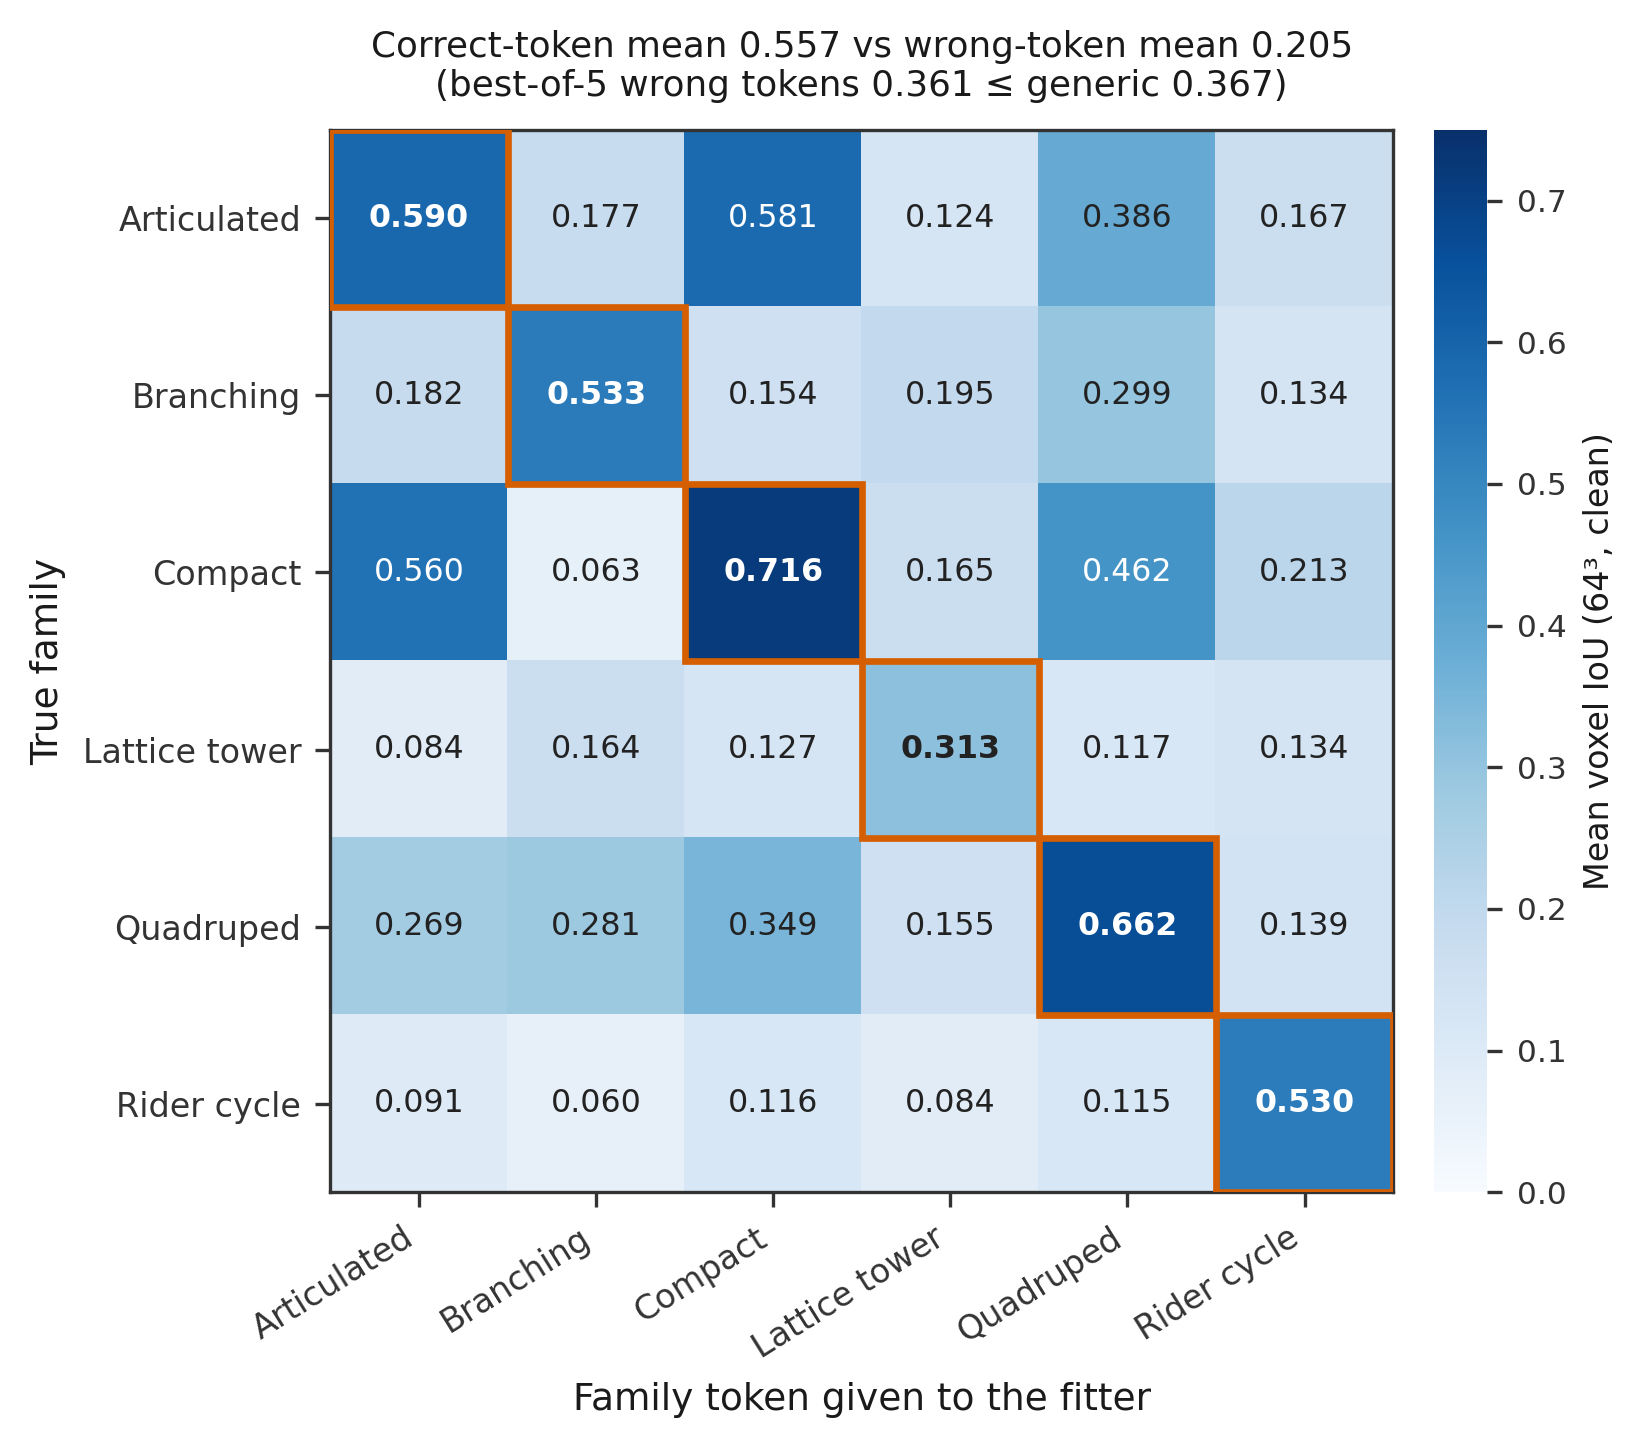
\includegraphics[width=\linewidth]{figures/fig_wrong_family_matrix.png}
\caption{Wrong-family analysis (clean condition, \(n{=}240\), mean voxel IoU).
Rows: true family; columns: family token supplied to the fitter. The diagonal
is the correct token. Off-diagonal cells fall below the diagonal and, with
few exceptions, also below the generic-graph mean of \(0.367\); the
exceptions cluster on the morphologically close vehicle families
(compact/articulated) and on the quadruped token applied to vehicle rows.}
\label{fig:wrong-family-matrix}
\end{minipage}\hfill
\begin{minipage}{0.44\linewidth}
\centering
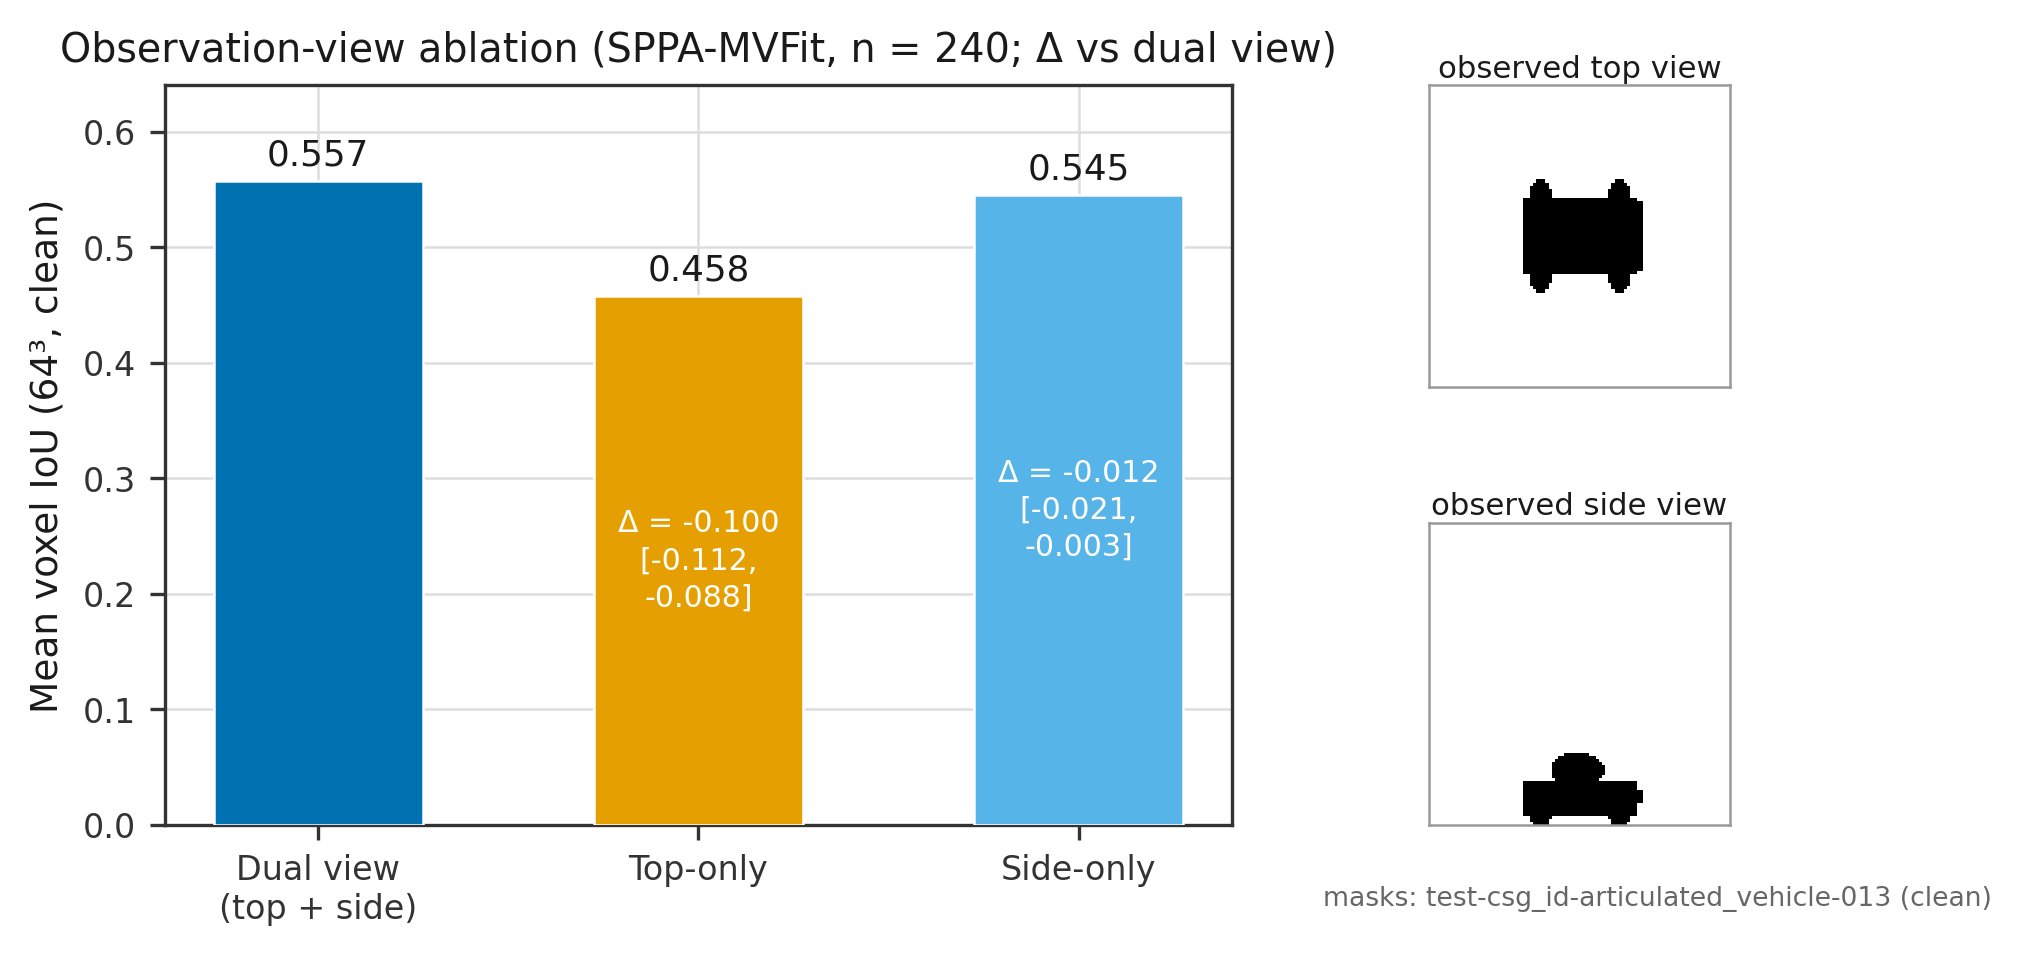
\includegraphics[width=\linewidth]{figures/fig_view_ablation.png}
\caption{View ablation of SPPA-MVFit (clean condition, \(n{=}240\), correct
family token): dual-view, top-only, and side-only mean voxel IoU with 95\%
bootstrap intervals.}
\label{fig:view-ablation}
\end{minipage}
\end{figure}

\subsection{Adversarial family instances}
\label{sec:adversarial}

A structural concern with the primary comparison is that it is nearly
guaranteed: the family graph encodes the same part topology that the CSG-ID
generators instantiate, so a positive H1 could be decided by design rather
than by measurement. The wrong-family arm already shows the prior can be
actively harmful; here we probe the complementary edge. A post-hoc
exploratory stratum of \(120\) adversarial actors (\(20\) per family, twelve
documented violation types, design frozen before measurement) keeps each
family's semantic class but violates its structural prior: rearward cabs,
split cargo beds, six-legged and asymmetric quadrupeds, out-of-order
platforms, a \(25^{\circ}\) leaning lattice tower, sidecar cycles, and cargo
over-scaled to \(250\%\) of the prior. Under the identical clean-mask
protocol, the paired SPPA advantage over Generic-MVFit falls from \(+0.209\)
on the same actors unviolated to \(+0.141\) (CI \([0.125,0.157]\)): violating
the prior destroys about one third of the advantage
(\(\Delta\Delta=-0.068\), CI \([-0.087,-0.048]\)) and SPPA-MVFit loses at
actor level in \(8.3\%\) of cases. Two violation types reach statistical
ties with both methods near the floor---the leaning tower (\(+0.009\), CI
\([-0.008,+0.026]\); a \(25^{\circ}\) shear is not expressible by
axis-aligned part scaling) and the cascade crown (\(+0.007\), CI
\([-0.015,+0.029]\))---while others leave the advantage intact or larger
(sidecar \(+0.320\)). The family prior is therefore neither a tautological
win nor a fragile one: its value degrades measurably and predictably with
prior violation, and the failure zones are identifiable
(Table in Supplementary Section~S.9).

\subsection{Ablations and sensitivity analyses}
\label{sec:ablations}

\paragraph{View ablation and side-view acquisition.}
\label{sec:view-ablation}
The objective consumes a top and a side silhouette. Refitting with only the
top view costs \(-0.100\) IoU (CI \([-0.112,-0.088]\)); refitting with only
the side view costs only \(-0.012\) (CI \([-0.021,-0.003]\))
(Figure~\ref{fig:view-ablation}). The side view carries nearly all of the 3D
information for this object envelope, and even the degraded top-only mode
(\(0.458\)) stays above dual-view Generic-MVFit (\(0.367\)) and the box
baselines. A side view is not available from a pure nadir pass: it requires an
oblique pass or orbit, or a second platform. The operational pipeline already
runs in a nadir footprint-only mode in production
(Section~\ref{sec:pipeline}); the top-only arm quantifies exactly that
degraded mode for the fitting path.


\paragraph{Oriented bounding box baseline.}
The primitive baselines are axis-aligned. A rotation-aware oriented bounding
box (top-mask minimum-area rectangle with gap-midpoint refinement, \(z\)
extent from the side mask) scores \(0.252\), practically identical to the
axis-aligned box (\(0.248\); paired difference \(-0.004\), CI
\([-0.005,-0.003]\)): the benchmark actors are presented axis-aligned, so
orientation freedom adds nothing, and SPPA-MVFit minus OBB is \(+0.306\) (CI
\([0.297,0.314]\); table in Supplementary Section~S.9). The box family of baselines, oriented or not, does not
close the representation gap. The wider representation design space is mapped
in Supplementary Section~S.1.

\paragraph{Generic-graph design sensitivity.}
\label{sec:generic-sensitivity}
Because the authors designed the generic graph (Section~\ref{sec:mvfit}),
three alternative generic graphs were registered in writing before any
measurement and evaluated under the same protocol: G2 (box/cylinder chassis),
G3 (vertical ellipsoid stack plus legs), and G4 (slot-wise mean of the six
family graphs, a fully mechanical rule). All three score \emph{below} the
original generic (table in Supplementary Section~S.9): against these
alternatives the measured SPPA advantage is, if anything, conservative.

\paragraph{Optimizer budget.}
The 31-candidate budget sits at the knee of the budget curve: 11 candidates
give \(0.528\) at \(3.6\)~ms mean, 21 give \(0.547\) at \(7.6\)~ms, the
adopted 31 give \(0.557\) at \(12.6\)~ms, and doubling to 61 gives \(0.560\)
at \(24.0\)~ms---a non-significant \(+0.002\) (CI \([-0.001,+0.005]\)) for
twice the compute (full sweep in Supplementary Section~S.9). Sweep timings
come from a separate post-hoc re-run on the same machine; IoU values are
bit-exact with the sealed run, which reports a \(9.4\)~ms median.

\paragraph{Role-aware IoU.}
Occupancy IoU does not test the role labels themselves. As a first
quantitative check, a slot-to-component mapping against the ground-truth
generators was frozen in writing before any computation and restricted
ex-ante to the CSG-ID stratum (\(120\) actors, 920 matched slot--component
pairs). Matched pairs reach \(0.545\) coverage and a role IoU of \(0.319\)
(Figure~\ref{fig:role-colored}b),
against \(0.053\) for a random-shuffle control (cyclic shuffle \(0.017\)): a
paired role-assignment advantage of \(+0.265\) (CI \([0.250,0.281]\); table in
Supplementary Section~S.9). This is
descriptive evidence on a frozen mapping over one stratum, not a confirmatory
endpoint.

\paragraph{Part-query task.}
To operationalize what role labels are worth, a part-query task was frozen in
writing before measurement on the same stratum: given a target role
(\emph{cargo}, \emph{wheels}, \emph{cab}, \emph{legs}, \emph{hitch},
\emph{platforms}), each method must return the voxels of that part. SPPA-MVFit
returns its role-labeled slot; controls are Generic-MVFit with its own slot
mapping and two frozen visual-hull heuristics (largest connected component;
lower half). Over 887 scorable queries (33 of 920 excluded for sub-voxel
ground truth, documented with a sensitivity analysis), SPPA-MVFit reaches
query F1 \(0.434\) versus \(0.145\) (generic), \(0.111\) and \(0.087\) (hull
heuristics), with normalized part-centroid error \(0.055\) versus
\(0.177\)--\(0.249\); the hull \emph{covers} (recall \(0.96\)) but cannot
\emph{select} (precision \(0.07\)). Structural part counting is exact in
\(70\%\) of actors versus \(0\%\) for the hull. The frontier is honest: the
largest-component heuristic \emph{wins} on fused branching crowns, the rider
fork scores zero, and lattice platform counts fail where graph arity and
ground truth disagree. Role value concentrates on small, numerous parts
(table in Supplementary Section~S.9).

\subsection{External sanity check on real meshes}
\label{sec:external-sanity}

As a post-hoc exploratory case study outside the design distribution, the
same methods were run on \(n{=}52\) real third-party meshes (Objaverse LVIS
subset and ModelNet40), mapped to the six families through a class-to-family
mapping frozen in writing before any evaluation and passed through visual
quality control (Table~\ref{tab:external-sanity};
Figures~\ref{fig:external-scatter} and~\ref{fig:external-gallery}). Mean fit
time remains millisecond-scale (\(9.8\)~ms per case, CPU). This is a sanity
check, not a benchmark: the sample is small, the class mapping is approximate,
and the evaluation reuses the synthetic-grid protocol on real geometry.

\begin{table}[H]
\centering
\scriptsize
\setlength{\tabcolsep}{3pt}
\caption{External sanity check on 52 real meshes
(voxel IoU at \(64^3\), clean condition; family headers abbreviated:
compact/articulated vehicle, branching vertical, lattice tower, rider cycle).
Mapping class-to-family frozen
before evaluation; per-family \(n\) in the table footer. The preregistered
\(+0.030\) margin does not replicate here (paired SPPA\(-\)Generic
\(+0.043\), CI \([-0.007,+0.094]\)).}
\label{tab:external-sanity}
% external sanity check (exploratory, post-hoc) - real meshes, clean condition
% voxel IoU (64^3) mean [95% bootstrap CI], seed 77157, 10000 resamples
\begin{tabular}{lrrrrrrr}
\toprule
Method & compact & articulated & quadruped & branching & lattice & rider & All \\
\midrule
\textbf{SPPA-MVFit} & \textbf{0.632} & \textbf{0.633} & \textbf{0.423} & \textbf{0.215} & \textbf{0.157} & \textbf{0.361} & \textbf{0.413} \\
Generic-MVFit & 0.508 & 0.319 & 0.393 & 0.382 & 0.288 & 0.288 & 0.370 \\
SPPA text-only & 0.449 & 0.188 & 0.242 & 0.058 & 0.101 & 0.172 & 0.213 \\
AABB & 0.577 & 0.593 & 0.386 & 0.244 & 0.368 & 0.259 & 0.411 \\
Ellipsoid & 0.613 & 0.527 & 0.496 & 0.369 & 0.470 & 0.398 & 0.485 \\
Capsule & 0.654 & 0.605 & 0.477 & 0.365 & 0.472 & 0.342 & 0.492 \\
Billboard & 0.164 & 0.070 & 0.256 & 0.111 & 0.077 & 0.333 & 0.172 \\
Visual hull & 0.809 & 0.783 & 0.715 & 0.462 & 0.581 & 0.530 & 0.656 \\
\midrule
\multicolumn{8}{l}{\footnotesize $n$ per family: compact=10, articulated=8, quadruped=10, branching=8, lattice=8, rider=8 (total 52).}\\
\multicolumn{8}{l}{\footnotesize Overall mean [CI95]: SPPA-MVFit 0.413 [0.359, 0.467]; Generic 0.370; Visual hull 0.656.}\\
\multicolumn{8}{l}{\footnotesize Paired SPPA$-$Generic: +0.043 [-0.007, +0.094].}\\
\bottomrule
\end{tabular}

\end{table}

\begin{figure}[H]
\centering
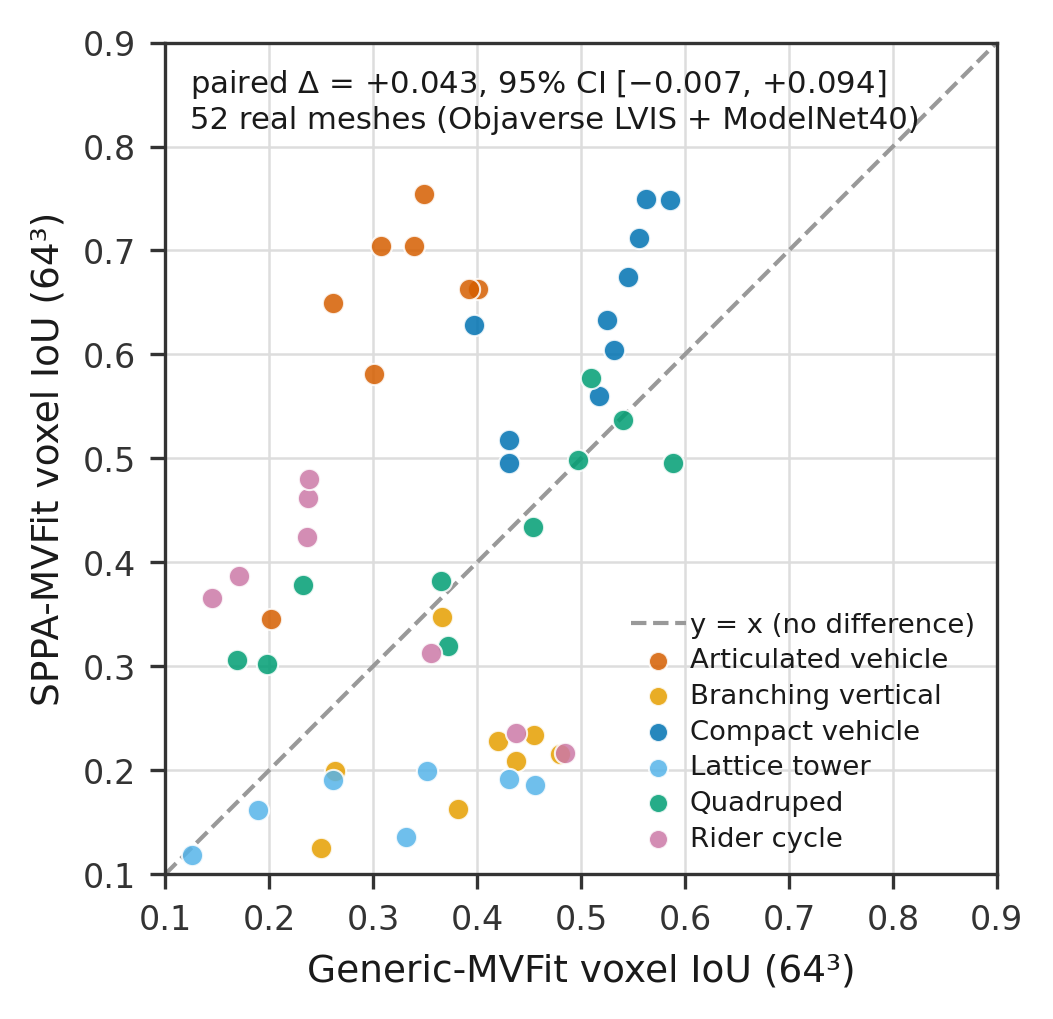
\includegraphics[width=0.55\linewidth]{figures/fig_external_scatter.png}
\caption{External sanity check: per-case SPPA-MVFit versus Generic-MVFit voxel
IoU on the 52 real meshes, colored by mapped family. Points near the diagonal
dominate; the paired difference (\(+0.043\), CI \([-0.007,+0.094]\)) includes
zero.}
\label{fig:external-scatter}
\end{figure}

\begin{figure}[H]
\centering
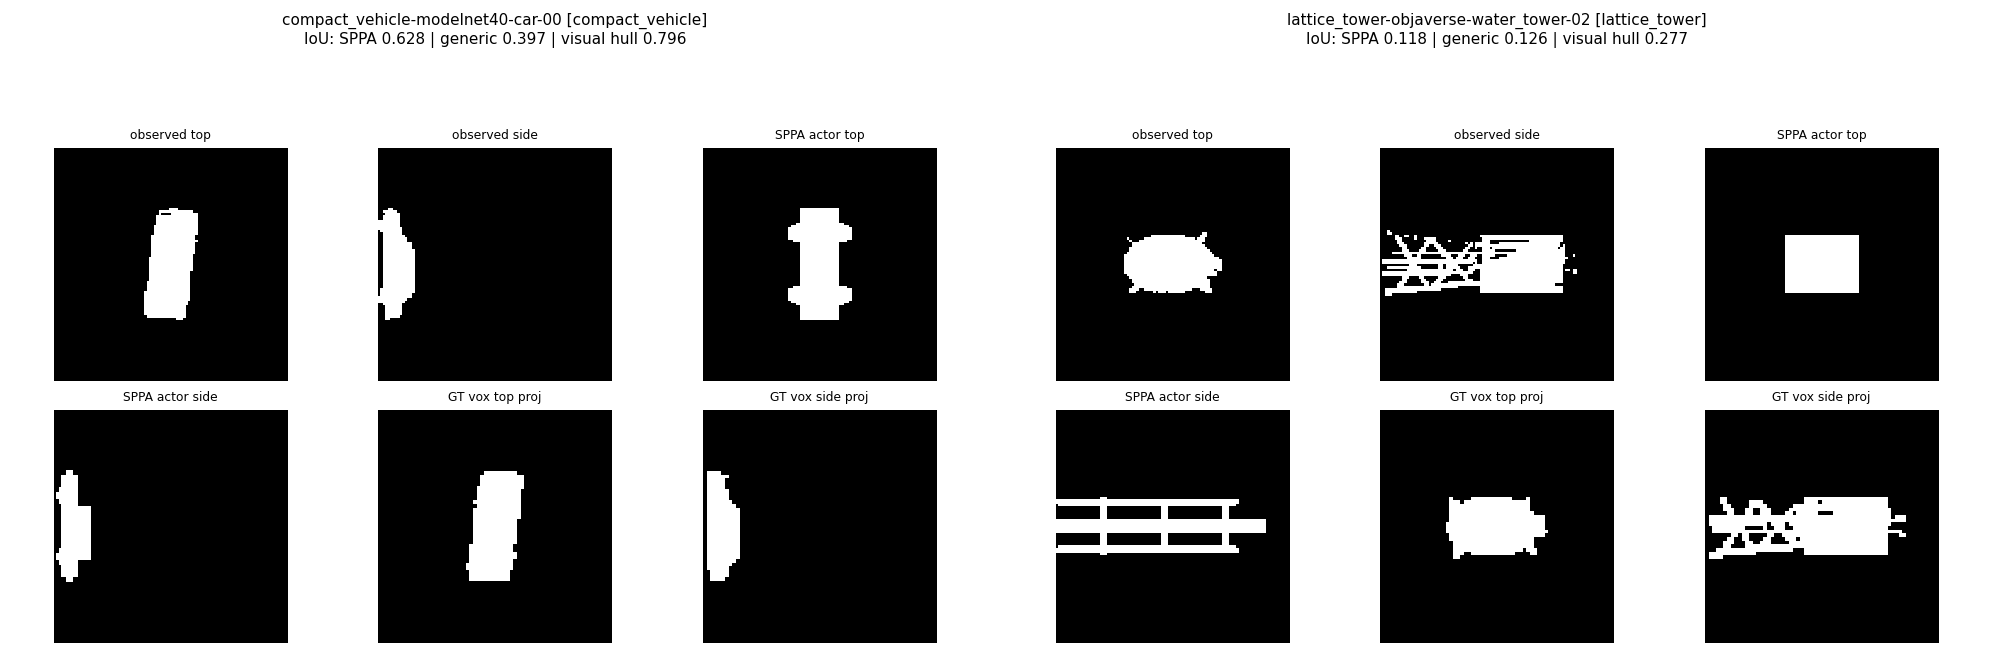
\includegraphics[width=\linewidth]{figures/fig_external_gallery.png}
\caption{External sanity check, qualitative. Left: a ModelNet40 car where
the family graph helps (SPPA 0.628 vs generic 0.397). Right: an Objaverse
water tower whose horizontal tank mismatches the vertical tower template
(SPPA 0.118 vs generic 0.126)---the template--instance mismatch failure
mode. Panels show observed masks, SPPA actor projections, and ground-truth
voxel projections.}
\label{fig:external-gallery}
\end{figure}

Three readings follow. First, the preregistered margin does not replicate on
external meshes at this sample size: SPPA-MVFit scores \(0.413\) (CI
\([0.359,0.467]\)) against Generic-MVFit \(0.370\) (CI \([0.335,0.405]\)), a
paired \(+0.043\) whose interval \([-0.007,+0.094]\) includes zero. Second,
the nonsemantic visual hull dominates raw occupancy with clean real
silhouettes (\(0.656\), CI \([0.606,0.704]\)), and the trivial geometric
primitives tell the same story: capsule (\(0.492\)), ellipsoid (\(0.485\)),
and even the axis-aligned box (\(0.411\)) match or exceed SPPA-MVFit
(\(0.413\)) here---outside the design distribution the family graph buys no
volumetric advantage over shape-free baselines, and the value of SPPA is the
semantic contract: role labels, bounded updates, and a telemetry-scale
payload. Third, the failure modes are informative and consistent with
Section~\ref{sec:wrong-family}: template--instance mismatch (horizontal water
towers fitted by a vertical tower graph), open geometry (bicycle wheel
spokes), and one LVIS mislabel retained as an out-of-distribution case (a
giraffe labeled \texttt{horse}). When the prior does not match, it hurts; the
contract's role is to detect that situation and degrade safely. Under mild
morphology corruption the pattern persists (SPPA \(0.380\), Generic
\(0.357\)).

\subsection{External neural generators: an input-modality mismatch demonstration}
\label{sec:neural-external-wave}

A secondary analysis, specified in writing before any measurement, compares
SPPA-MVFit with two measured external neural image-to-3D generators,
TripoSR~\cite{tochilkin2024triposr} and
Hunyuan3D-2mini-turbo~\cite{zhao2025hunyuan3d}, on sixty of the held-out cases
(Figure~\ref{fig:pareto-neural}; full table and protocol in Supplementary
Section~S.2). Each generator received two inputs: a clean-crop shaded oblique
render, its best condition, and the raw \(96\times96\) top telemetry mask, the
closest visual analog of the channel SPPA consumes. On these cases SPPA-MVFit
reaches \(0.561\) mean voxel IoU at \(9.2\)~ms CPU with a 1.45~kB update
descriptor, against \(0.128\)--\(0.231\) for the measured neural outputs,
whose meshes carry \(28\)k--\(3.1\)M triangles and MB-scale payloads on an
RTX~5090. Two observations sharpen the boundary. First, both generators score
\emph{higher} from the harsh top mask than from their generous clean-crop
render: single-view image-to-3D models hallucinate occluded structure, whereas
a calibrated footprint constrains occupancy directly---telemetry-shaped
evidence is not a degraded image but a different measurement channel. Second,
the wave measures one operating point per system under deliberately asymmetric
input channels: Hunyuan3D-2mini-turbo is a distilled mini/turbo checkpoint,
not the flagship model of its family, and the comparison is not an
image-to-3D leaderboard.

\begin{figure}[H]
\centering
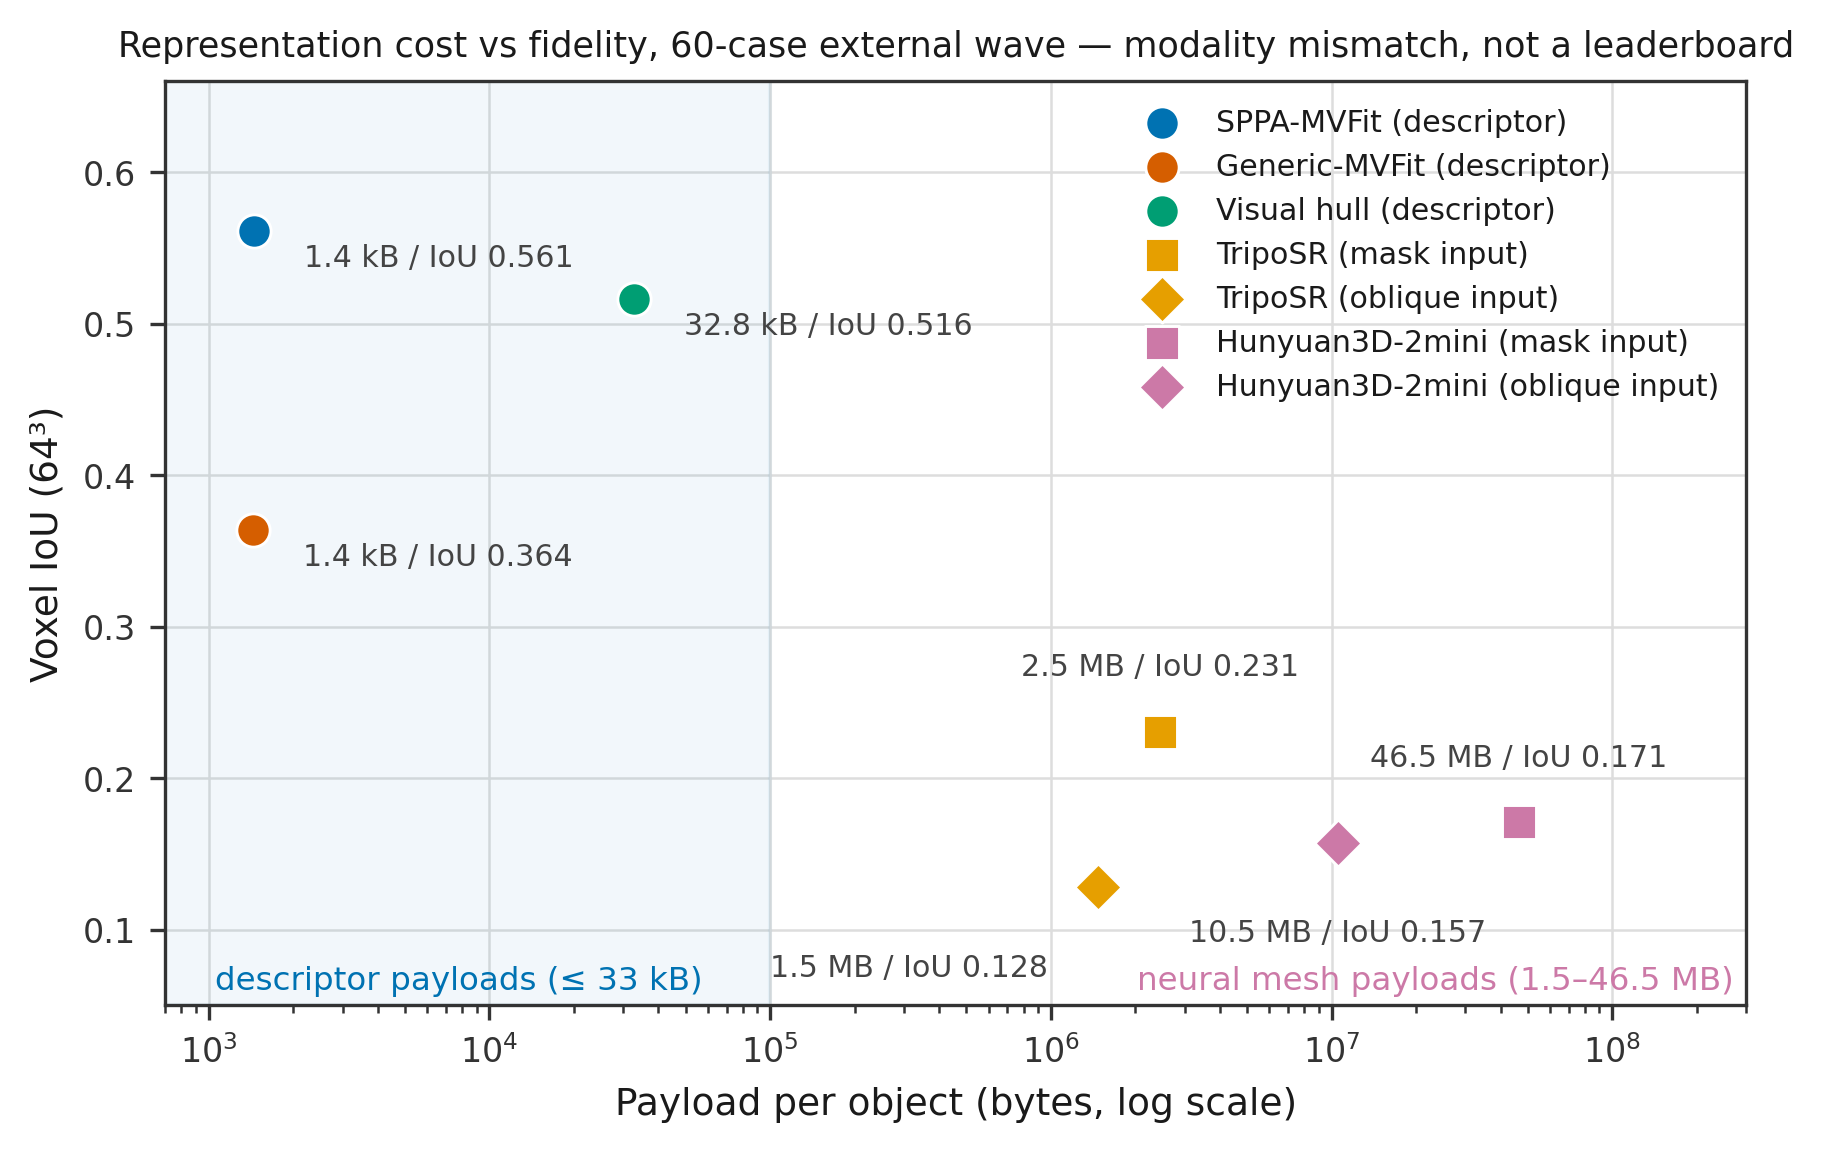
\includegraphics[width=0.6\linewidth]{figures/fig_pareto_neural.png}
\caption{Operating-point comparison on sixty held-out cases: mean voxel IoU
against per-object payload in bytes (log scale) for SPPA-MVFit, Generic-MVFit,
visual hull, and the measured neural generators under both input conditions.
SPPA rows are CPU-only and their payload is the update descriptor, not a
mesh; the juxtaposition is an input-modality mismatch shown for
operating-point context, not a leaderboard.}
\label{fig:pareto-neural}
\end{figure}

\subsection{Real-image probes and deployment runtime}
\label{sec:deployment-summary}

Four real-image probes exercise the dual-input contract of
Section~\ref{sec:pipeline} (Figure~\ref{fig:probes-grid}): a YOLOE-26s
open-vocabulary detector supplies approximate semantic evidence on the image
path, while the tag path uses reviewed text only. Detector evidence is not
treated as ground truth: weak labels are refined only to conservative
families (YOLOE's \texttt{vehicle} on the tractor-trailer crop becomes
\texttt{articulated\_vehicle}, never the reviewed \texttt{tractor\_trailer}
class), implausible footprint aspect ratios are clamped by family priors, and
unsafe image-derived pose is withheld from the runtime descriptor. A 20-label
verifier-gated open-label probe accepts 16/20 labels into reviewed families
with 8/20 verified recipes (Supplementary Section~S.3), and a
role-preservation diagnostic keeps cab and wheel priors fixed while cargo
length changes (Supplementary Section~S.5). Per-probe evidence, replay
audits, and input-mode ablations are in Supplementary Section~S.4; no 3D
ground truth exists for these images, so no IoU is reported for them.

\begin{figure}[H]
\centering
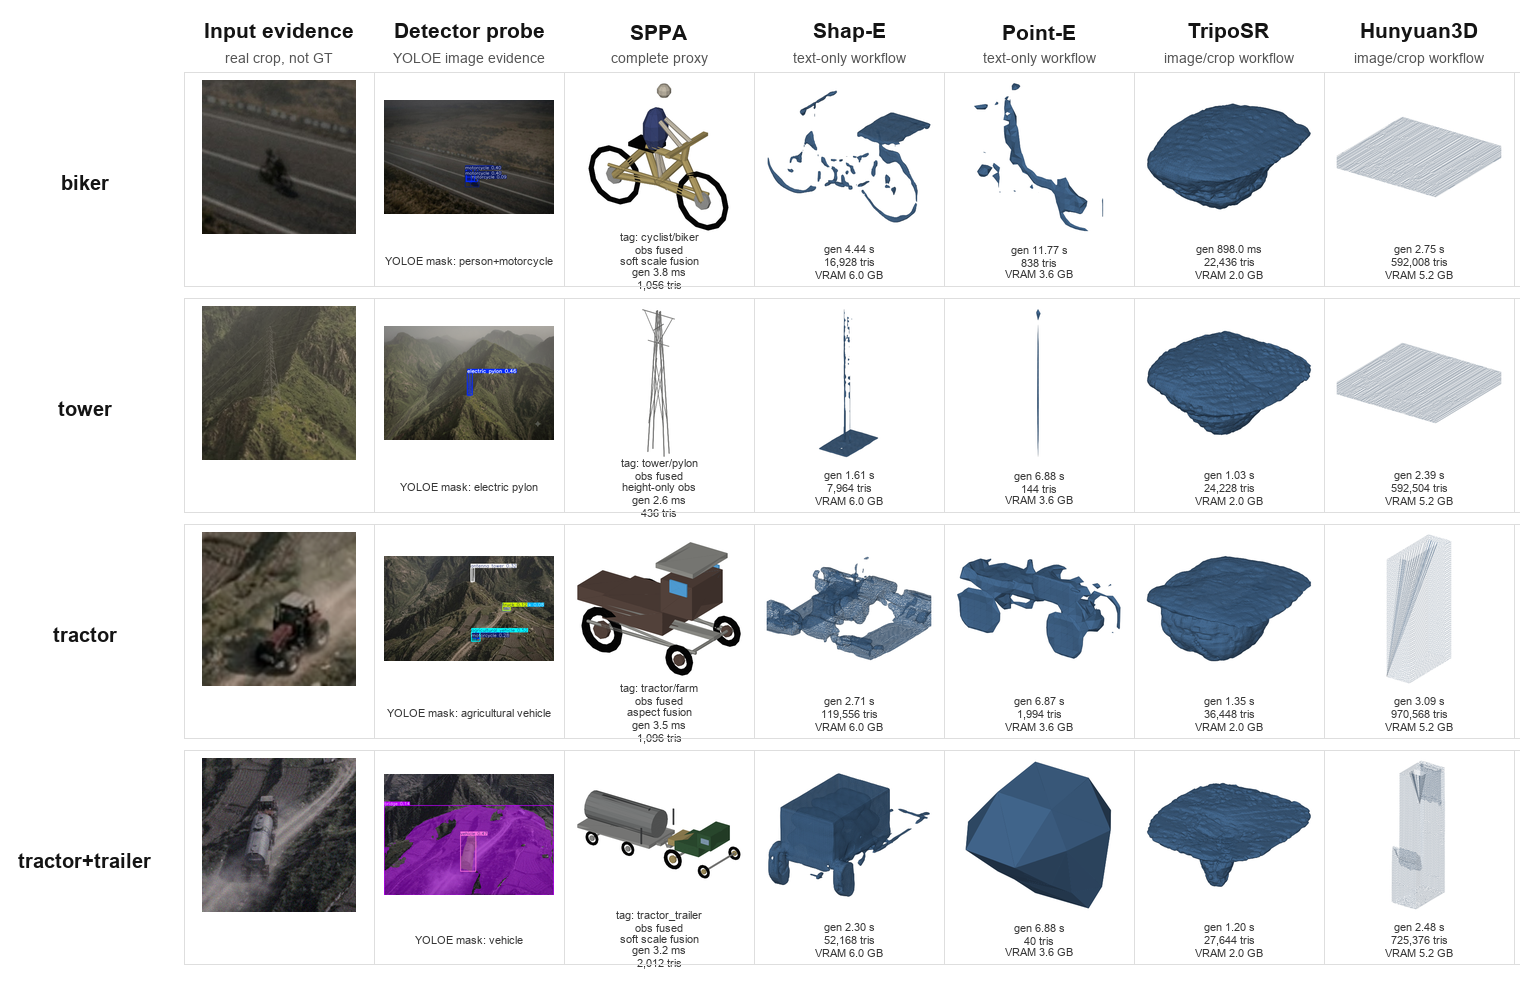
\includegraphics[width=0.8\linewidth]{figures/fig_probes_grid.png}
\caption{Real-image probes for biker, electrical tower, tractor, and
tractor-with-trailer (rows). Columns: input crop, YOLOE detector evidence,
the emitted SPPA proxy, and four reproduced text/image-to-3D baselines
(Shap-E, Point-E, TripoSR, Hunyuan3D) annotated with generation time,
triangle count, and VRAM. Detector output is evidence, not ground truth;
the neural columns receive a single image or crop, an input-modality
mismatch shown for operating-point context, not a ranking.}
\label{fig:probes-grid}
\end{figure}

The deployment layer is the descriptor/update contract consumed by the
optional Unreal Engine 5.7 backend. Table~\ref{tab:deployment-runtime-summary}
condenses the runtime evidence and Figure~\ref{fig:runtime-scaling} the
packaged scaling behavior; the full Unreal/HISM matrix with run identifiers is
Supplementary Section~S.8. Packaged replay at 100 synthetic objects passes a
33.3~ms desktop frame budget but misses 60~FPS; dense shape updates remain the
limiting factor even under HISM batching, and curated assets remain preferable
when a matched asset exists (shape-stream P95 \(6.789\)~ms vs.\ \(22.445\)~ms
on the two-label cow/tower subset).

\begin{table}[H]
\centering
\footnotesize
\setlength{\tabcolsep}{3pt}
\renewcommand{\arraystretch}{1.12}
\caption{Condensed deployment runtime evidence (run identifiers omitted here;
full matrix in Supplementary Section~S.8). Python contract timings are not
Unreal frame times, and packaged runs are short synthetic replays, not live
flight telemetry.}
\label{tab:deployment-runtime-summary}
\begin{tabularx}{\linewidth}{@{}L{0.30\linewidth}Y Y@{}}
\toprule
Evidence & Summary value & Boundary \\
\midrule
Descriptor build (81,568-row replay) & P50/P95 \(391.8/515.0\)~\(\mu\)s & Python contract cost, not frame time \\
Update-packet build & P50/P95 \(16.8/75.3\)~\(\mu\)s & Python contract cost \\
Scheduler decision & P50/P95 \(9.2/14.2\)~\(\mu\)s & Python contract cost \\
Editor-Cmd and packaged recorded replay & 27/27 payload applications accepted & recorded streams, no live network \\
Packaged 100-object replay & pose/shape frame P95 \(17.814/19.256\)~ms & desktop feasibility; misses 60 FPS P95 \\
Packaged HISM partial update, 500 objects & pose/shape frame P95 \(16.528/29.787\)~ms & 10\% changed-track synthetic schedule \\
\bottomrule
\end{tabularx}
\end{table}

\begin{figure}[H]
\centering
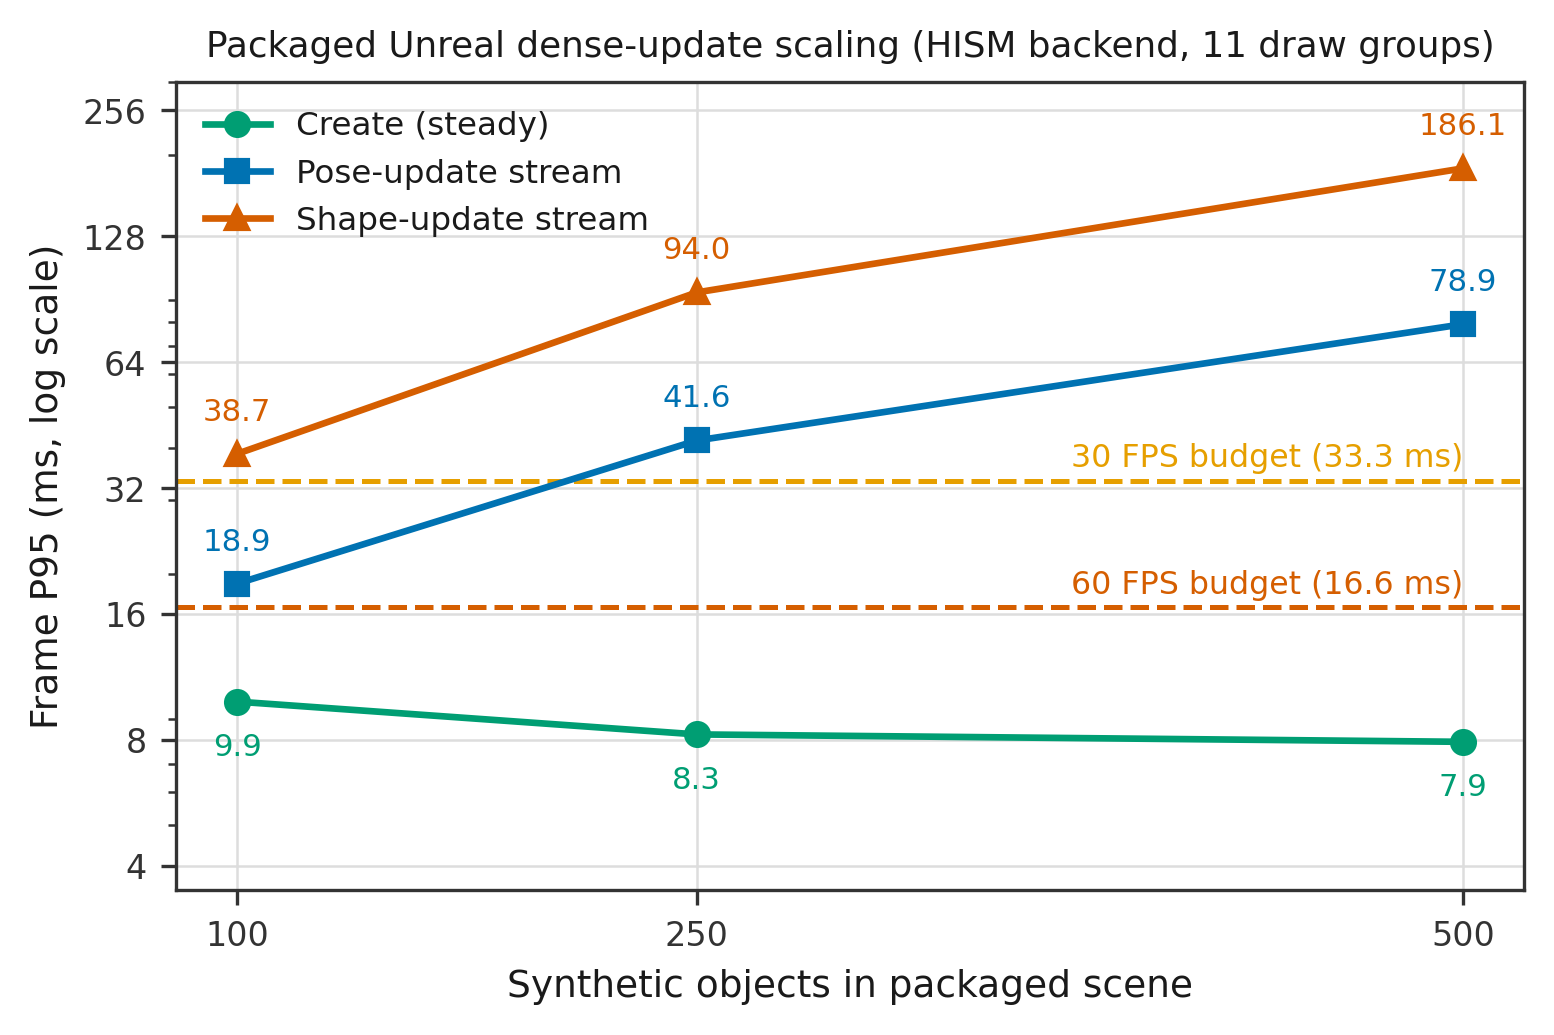
\includegraphics[width=0.5\linewidth]{figures/fig_runtime_scaling.png}
\caption{Packaged-runtime scaling (HISM backend, dense-update streams):
frame P95 versus object count for the create, pose-update, and shape-update
streams. The 33.3~ms line marks a desktop 30~FPS budget; dense shape updates
exceed it already at 100 objects and dense pose updates between 100 and 250,
while the sparse 10\% changed-track schedule of
Table~\ref{tab:deployment-runtime-summary} stays below it at 500 objects.}
\label{fig:runtime-scaling}
\end{figure}

\subsection{A real detector stream case study}
\label{sec:real-stream}

The motivating scenario is a real detector running on a live georeferenced
twin. As a post-hoc exploratory case study, a recorded 1{,}394-frame flight
stream over the Ejea twin was re-analyzed end to end: a custom YOLO detector
with real confidence noise and real confusions (cows hallucinated on tower
textures), MAVLink telemetry, and exact simulator ground truth for the
static tower anchors. Detections with locked telemetry yield 1{,}902 cases
(308 tower, 848 cow, 746 biker detections). Every method receives the
identical observation---an oriented ground footprint geo-projected from the
detection box plus a monocular height estimate---so the comparison carries
no input advantage, and wrong detector tokens are kept as a natural
condition.

Three findings bound the operating point honestly
(Table~\ref{tab:real-stream}; Figure~\ref{fig:real-stream}). First,
localization is observation-bound, not fitter-bound: all methods sit at
\(\approx\)\(33\)~m median 3D error, exactly on the identity line of
footprint-center error versus anchor error, because the low-altitude stream
(AGL 10--23~m) compresses monocular range; footprint IoU against a
\(5{\times}5\)~m base is degenerate for every method. Second, SPPA-MVFit
does \emph{not} win the 2D reprojection metric on real evidence (\(0.298\)
median versus \(0.42\)--\(0.45\) for box proxies): the family prior buys 3D
part structure at the cost of image overlap when the monocular height
estimate conflicts with the prior bounds (a \(13.75\)~m tower column versus
a \(\approx\)\(5\)~m observed extent). The stream carries no 3D ground
truth, so the quantity the sealed benchmark measures---3D occupancy---cannot
be scored here; what the stream adds is precisely the evidence-versus-prior
tension that a ground-truth benchmark cannot see. Third, the tension is
quantifiable: on the 138 GT-matched cases where the real detector emitted a
wrong family token, refitting with the correct token collapses the 2D fit
from \(0.381\) to \(0.025\)---the correct prior cannot explain the
misleading evidence that triggered the wrong label (token-arm table in
Supplementary Section~S.9). Fit latency (\(11.8\)~ms median) stays far below
the 2--15~Hz stream rate, so the operating point is computationally viable
even in this degraded mode.

We read this study as the field counterpart of the boundary map: in
production the system should run the footprint-only mode declared in
Section~\ref{sec:pipeline} (and quantified by the top-only arm), reserve
dual-view fitting for oblique passes, and treat detector-token confidence
as a routing signal rather than a given.

\begin{table}[H]
\centering
\scriptsize
\setlength{\tabcolsep}{3pt}
\caption{Real detector stream case study (exploratory post-hoc, not sealed):
1{,}902 detections from a 1{,}394-frame flight over the georeferenced twin
with a real custom detector, real telemetry, and exact tower-anchor ground
truth. Localization and footprint columns: GT-matched subset (\(n{=}217\);
wrong detector tokens kept as a natural condition); reprojection and
latency: all cases. All methods are observation-bound at \(\approx\)\(33\)~m;
SPPA-MVFit trades 2D image overlap for 3D part structure (the stream has no
3D ground truth).}
\label{tab:real-stream}
% E7 Real Stream Wave - exploratory post-hoc (not confirmatory). MAIN-TEXT version.
% Loc./footprint columns: GT-matched subset (n=217, tower anchors; wrong detector
% tokens kept as a natural condition). Reprojection/latency: all n=1902 cases.
\begin{tabular}{@{}lccccc@{}}
\toprule
Method & Loc. err. 3D med. (m)$^{\dagger}$ & Footprint IoU$^{\dagger}$ & 2D reproj. IoU med. [P25, P75] & Latency (ms) \\
\midrule
SPPA-MVFit (this work) & 32.8 & 0.000 & 0.298 [0.218, 0.392] & 11.8 \\
Generic-MVFit & 32.8 & 0.000 & 0.423 [0.394, 0.448] & 13.4 \\
OBB & 32.7 & 0.000 & 0.446 [0.398, 0.492] & 0.22 \\
AABB & 32.7 & 0.000 & 0.330 [0.299, 0.357] & 0.25 \\
Visual hull (non-semantic) & 32.7 & 0.000 & 0.446 [0.398, 0.493] & 0.50 \\
Capsule & 32.7 & 0.000 & 0.445 [0.422, 0.466] & 1.31 \\
\bottomrule
\end{tabular}

\end{table}

\begin{figure}[H]
\centering
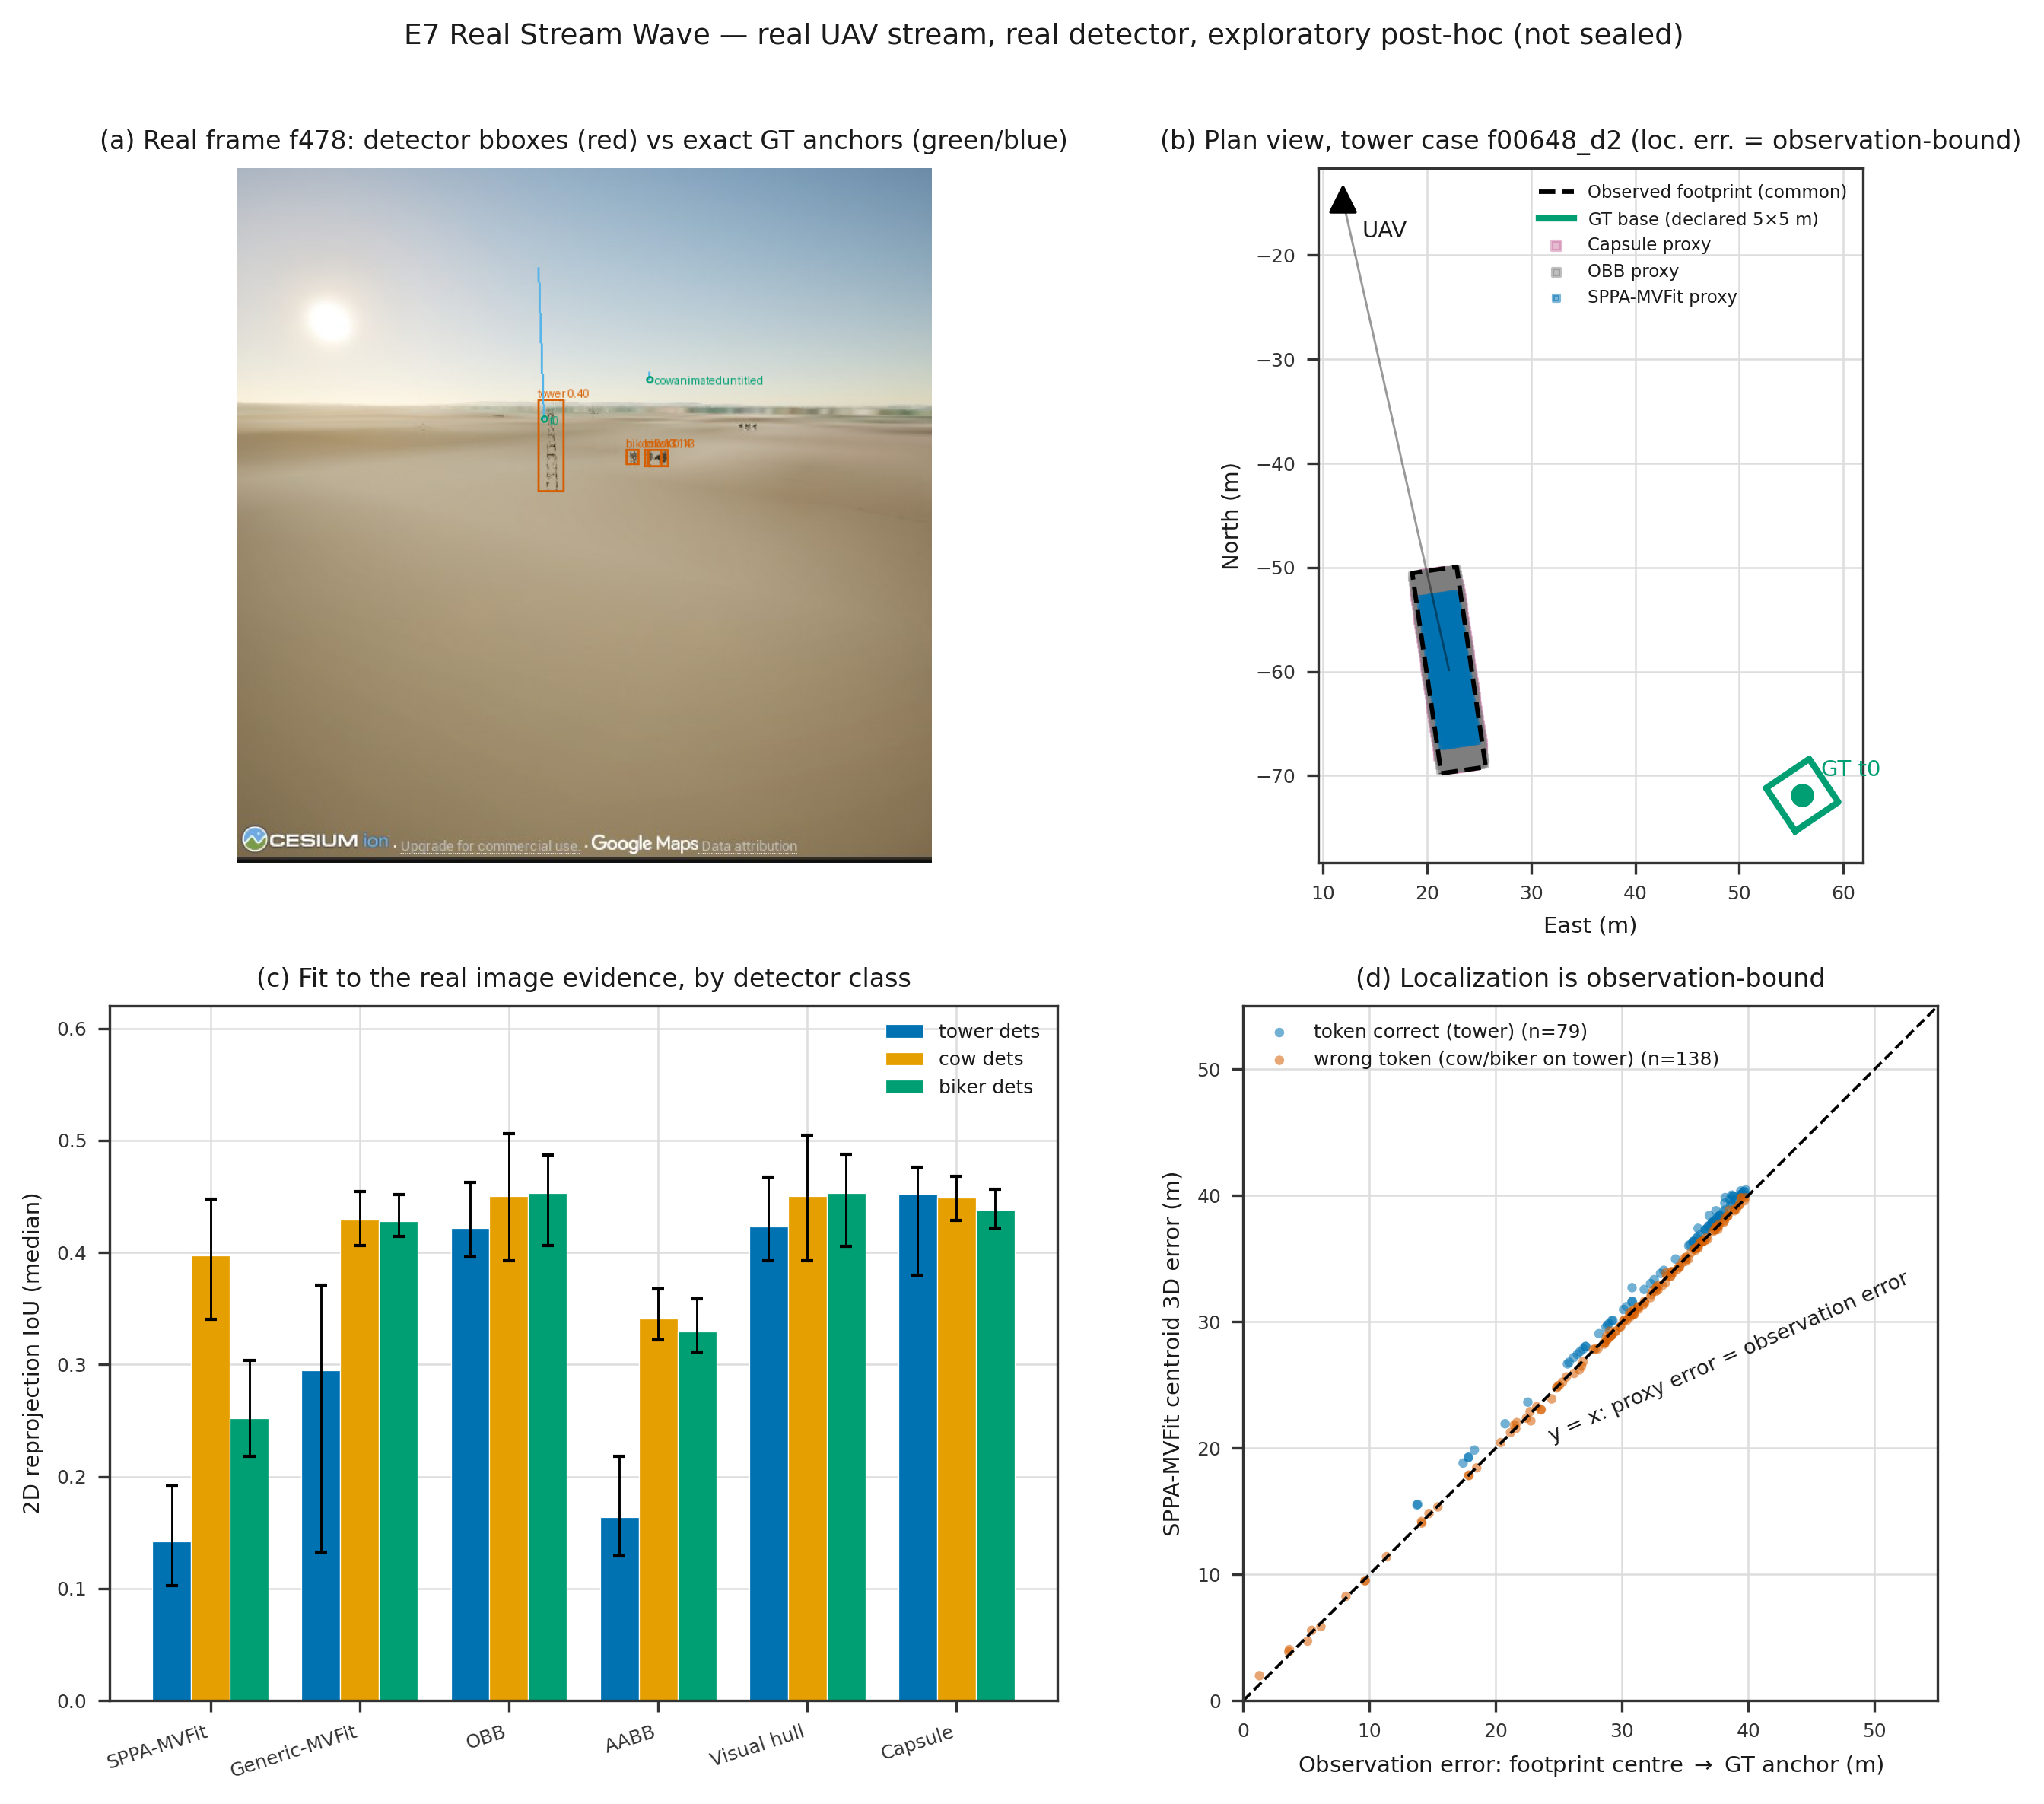
\includegraphics[width=0.82\linewidth]{figures/fig_real_stream.png}
\caption{Real stream case study. (a)~Frame 478 with detector boxes and exact
ground-truth anchors. (b)~Plan view of a tower case: the observed footprint
(dashed) and all fitted proxies sit \(\approx\)\(35\)~m from the exact
anchor---observation-bound. (c)~2D reprojection IoU by detector class.
(d)~Fitted-centroid error versus observation error: the identity line holds
for all methods.}
\label{fig:real-stream}
\end{figure}

\section{Discussion}
\label{sec:discussion}

The confirmatory result answers the preregistered question: under identical
calibrated silhouettes and optimizer budget, a frozen family part graph
improves lightweight occupancy over a generic eight-part graph by a large and
stable margin. The decomposition of
Section~\ref{sec:results-decomposition} shows that the knowledge
representation, not a clever optimizer, is the active ingredient; secondary
gains over text-only SPPA show that silhouette evidence helps when the same
family graph is held fixed.

The boundary analyses are as informative as the headline. A wrong family token
is worse than no prior at all, which turns fallback routing from an
engineering convenience into a measured requirement. The adversarial stratum
shows the advantage is killable rather than tautological: violating the
structural prior while preserving the semantic class destroys a third of the
effect and produces identifiable tie zones where no axis-aligned part graph
can win. The side view carries
nearly all of the 3D information, yet it is unavailable from a pure nadir
pass: acquiring it requires an oblique pass, an orbit, or a second platform,
and otherwise the system degrades to the footprint-only mode that already runs
in production---quantified by the top-only arm, which still beats the generic
dual-view fit. On external real meshes the margin does not transfer and
shape-free baselines match or exceed SPPA on raw occupancy; what remains
differentiating outside the design distribution is the contract---role labels,
bounded updates, and a telemetry-scale payload---not volumetric leadership.
Visual hull can approach SPPA-MVFit IoU because it is free to materialize
denser occupancy without an eight-part role-labeled actor contract; the
part-query task quantifies what that contract buys, since the hull covers but
cannot select (query F1 \(0.434\) versus \(0.111\)). Finally, the real
detector stream relocates the bottleneck entirely: under monocular
low-altitude observation every method is observation-bound, and the family
prior trades image overlap for 3D structure---so deployment should route
between footprint-only and dual-view modes rather than treat fitting as
always-on.

\label{sec:threats}Several threats to validity remain binding. The primary
comparison is structurally favored by design: the family graphs encode the
same part topology that the CSG-ID generators instantiate, so preregistration
quantifies the effect but cannot make it surprising---the load-bearing
evidence that the advantage is real, killable, and bounded is the boundary
map (wrong-family arm, adversarial stratum, external meshes, real stream),
not H1 alone. The held-out
set is synthetic and developer-held-out; positive OOD-stratum differences do
not license claims about real UAV masks, detectors, or metric flight geometry.
Family tokens are supplied, so the experiment is family-conditioned rather
than open-set. Silhouettes are clean orthographic projections plus
prespecified corruptions, not real detector masks. Timing is local CPU
wall-clock for the fitter, not flight-laptop Unreal frame time, and the
packaged replay evidence consists of short synthetic streams, not live
telemetry or VR readiness. The real-stream study is a single recorded flight
with one custom detector, monocular low-altitude views, no 3D ground truth,
and 2D reprojection metrics only; its localization errors reflect the
observation model, not the fitter, and its tower-anchor subset is small. The same team authored the family graphs and the
generic competitor; the sensitivity variants of
Section~\ref{sec:generic-sensitivity} bound, but do not eliminate, the
resulting baseline-design risk. Within these boundaries the supported claim is
narrow: on the held-out synthetic test, family conditioning improves occupancy
beyond the prespecified margin; the shared generator supports text-only and
silhouette-fitted modes; and SPPA descriptors can be consumed by an optional
Unreal backend that coexists with curated assets. Real-UAV reconstruction
accuracy, universal open-set geometry, operator benefit, and neural
image-to-3D ranking remain outside the claim.

Three directions are left to future work. First, the frozen coordinate-descent
fitter could be replaced by population-based or differentiable-rendering
fitting, and the iterative fit could be amortized by a small learned
mask-to-\(\theta\) predictor, keeping the representation and contract while
moving per-case cost toward microseconds; the primitive vocabulary could
likewise be extended toward superquadrics. Second, the external gap measured
here calls for public real-data tests with metric ground truth and
detector-derived silhouettes rather than assumed calibration. Third, any
operator-facing benefit must be evaluated with human-factors methods such as
SAGAT and NASA-TLX \cite{endsley1988sagat,endsley1995situation,hart1988nasatlx};
the present paper contains no pilot study.

\section{Conclusion}

Family-conditioned SPPA-MVFit shows that a reviewed semantic part graph is a
measurable occupancy prior for lightweight multiview proxy fitting. Under a
preregistered equal-budget comparison, SPPA-MVFit improves clean 3D occupancy
over Generic-MVFit by \(0.190\) absolute IoU (95\% CI \([0.181,0.199]\)) on
240 held-out synthetic actors, with positive strata and millisecond-scale
local cost. Most of the advantage is the family-graph representation rather
than the fitter; a wrong family token is worse than no family prior at all;
and the margin does not transfer unchanged to real meshes whose instances
mismatch the templates. Adversarial instances that violate the structural
prior destroy a third of the advantage and expose identifiable tie zones,
while a real detector stream with exact anchor ground truth relocates the
field bottleneck in the monocular observation itself. The durable contribution is the
contract---family-conditioned roles, bounded updates, and a telemetry-scale
payload---whose part-query value is measured (query F1 \(0.434\) versus
\(0.111\) for occupancy-only controls), together with a quantified occupancy
envelope that holds inside the
design distribution. The next steps are external public data with metric
ground truth, detector-derived silhouettes, and, only if claimed, operator
studies.

\section*{Data Availability}

The SPPA-MVFit reproducibility package, protocol amendments, NIST-bound seed
manifest hashes, and confirmatory summaries are included under
\texttt{reproducibility/sppa\_mvfit/}. Large Unreal artifacts and historical
engineering logs remain supporting material and are not required to recompute
the primary H1 tables.

\section*{Code Availability}

The fitting, evaluation, and table-export code used to produce the reported
results is part of the reproducibility package above and will be released in a
public repository upon publication.

{\footnotesize
\bibliographystyle{plain}
\bibliography{semantic_proxy_3d_references}
}

\end{document}
